% % % % % % % %  MDT UFSM 2015  % % % % % % % % 
%% Arquivo base para o documento - ver. 1.08 %%
% % % % % % % % % % % % % % % % % % % % % % % % 


% % % OPCOES DE COMPILACAO
% % % PAGINACAO
% % % PAGINACAO SIMPLES (FRENTE): PARA TRABALHOS COM MENOS DE 100 PAGINAS
\documentclass[oneside,openright,12pt]{ufsm_2015} %%%%% OPCAO PADRAO -> PAGINACAO SIMPLES. PARA TRABALHOS COM MAIS DE 100 PAGINAS COMENTE ESTA LINHA E DESCOMENTE A LINHA 
% % % % % % % % % % % % % % % % % % % % % % % % % % % % % % % % % % % % % % %
% PAGINACAO DUPLA (FRENTE E VERSO): PARA TRABALHOS COM MAIS DE 100 PAGINAS
% \documentclass[twoside,openright,12pt]{ufsm_2015}  %%%% PARA TRABALHOS COM MAIS DE 100 PAGINAS DESCOMENTE AQUI
% % % % % % % % % % % % % % % % % % % % % % % % % % % % % % % % % % % % %


% % % %  CODIFICACAO DO TEXTO 
% % % %  POR PADRAO USA-SE UTF8. PARA APLICAR A CODIFICACAO OESTE EUROPEU (ISO 8859-1) DESCOMENTE A LINHA ABAIXO. ELA ATIVA A OPCAO "latin1" DO PACOTE "inputenc"
% \oesteeuropeu
% % % % % % % % % % % 

% % % % % % % % PACOTES PESSOAIS % % % % % % % %  
\usepackage{lipsum}
\usepackage{listings}
\usepackage{xcolor}






%\usepackage[ruled, longend]{algorithm2e}

% % % % % % % % DEFINICOES PESSOAIS % % % % % % % %
\newcommand{\ignore}[2]{\hspace{0in}#2}
\newcommand\tab[1][0.75cm]{\hspace*{#1}}
% % % % % % % % % % % % % % % % % % % % % % % % % % % % % % % % % % % % % % % % % % % 


% % % % % % % % % % % % % % % % % % % % % % % % % % % % % % % % % 
% % % % % % % % % % % % DADOS DO TRABALHO % % % % % % % % % % % % 
% % % % % % % % % % % % % % % % % % % % % % % % % % % % % % % % % 

% % % % % % % % % % INFORMACOES INSTITUCIONAIS % % % % % % % % % % 


% % CENTRO DE ENSINO DA UFSM
\centroensino{Centro de Tecnologia}  %%% NOME POR EXTENSO
\centroensinosigla{CT}  %%% SIGLA

% % CURSO DA UFSM
\nivelensino{Bacharelado}  %%%%%%% NIVEL DE ENSINO 
\curso{Ciência da Computação }   %%%%% NOME POR EXTENSO
%\ppg{PPGALGO}   %%%%%% SIGLA
\statuscurso{Curso}  %%%% STATUS= {Programa} ou {Curso}
% \EAD  %%%% para cursos EAD
% % % %  LOCAL DO CAMPUS OU POLO
\cidade{Santa Maria}
\estado{RS}

% % % % % % % % % % INFORMACOES DO AUTOR % % % % % % % % % % 
\author{Pedro Langbecker Lima}   %%%%% AUTOR DO TRABALHO
\sexo{M} %%%% SEXO DO AUTOR -> M=masculino   F=feminino (IMPORTANTE PARA AJUSTAR PAGINAS PRE-TEXTUAIS)
\grauensino{Bacharelado}    %%%%%%%% GRAU DE ENSINO A SER CONCLUIDO
\grauobtido{Bacharel}    %%%%% TITULO OBTIDO
\email{plima@inf.ufsm.br}   %%%% E-MAIL PARA CATALOGRAFICA (COPYRIGHT) - OBRIGATORIO
%\endereco{Rua das abobrinhas, n. 666} %%%% TELEFONE PARA CATALOGRAFICA (COPYRIGHT) (CAMPO OPICIONAL -- CASO NAO POSSUA OU NAO QUEIRA DIVULGAR COMENTE A LINHA)
%\fone{11 2222 3333}   %%%% TELEFONE PARA CATALOGRAFICA (COPYRIGHT) FORMATO {11 2222 3333} (CAMPO OPICIONAL -- CASO NAO POSSUA OU NAO QUEIRA DIVULGAR COMENTE A LINHA)
%\fax{11 2222 3333}   %%%% FAX PARA CATALOGRAFICA (COPYRIGHT) FORMATO {11 2222 3333} (CAMPO OPICIONAL -- CASO NAO POSSUA OU NAO QUEIRA DIVULGAR COMENTE A LINHA)


% % % % % % % % % % INFORMACOES DA BANCA % % % % % % % % % % 
% OBSERVACOES: O CAMPO ORIENTADOR EH OBRIGATORIO E NAO DEVE SER COMENTADO
% % % % % %    OS DEMAIS MEMBROS DA BANCA (COOREIENTADOR E DEMAIS PROFESSORES) QUANDO COMENTADOS NAO APARECEM NA FOLHA DE APROVACAO (O LAYOUT DA FOLHA DE APROVACAO ESTA PREPARADO PARA O ORIENTADOR E ATE MAIS 4 MEMBROS NA BANCA
\orientador{João Vicente Ferreira Lima}{Dr}{UFSM}{M}{M}  %%%INFORMACOES SOBRE ORIENTADOR: OS CAMPOS SAO:{NOME}{SIGLA DA TITULACAO}{SIGLA DA INSTITUICAO DE ORIGEM}{SEXO} M=masculino   F=feminino {PARTE DA BANCA?} P=presidente  M=Membro  N=Nao faz parte
%\coorientador{Co-orientadora placeholder}{Dra}{UFSM}{F}{M} %%%INFORMACOES SOBRE CO-ORIENTADOR: OS CAMPOS SAO:{NOME}{SIGLA DA TITULACAO}{SIGLA DA INSTITUICAO DE ORIGEM}{SEXO} M=masculino   F=feminino {PARTE DA BANCA?} P=presidente  M=Membro  N=Nao faz parte
\bancaum{Carlos Raniery Paula dos Santos}{Dr}{UFSM}{M}{M}  %%%INFORMACOES SOBRE PRIMEIRO NOME DA BANCA: OS CAMPOS SAO:{NOME}{SIGLA DA TITULACAO}{SIGLA DA INSTITUICAO DE ORIGEM}{SEXO} M=masculino   F=feminino {PARTE DA BANCA?} P=presidente  M=Membro  N=Nao faz parte
\bancadois{Sérgio Luís Sardi Mergen}{Dr}{UFSM} %%%INFORMACOES SOBRE SEGUNDO NOME DA BANCA: OS CAMPOS SAO:{NOME}{SIGLA DA TITULACAO}{SIGLA DA INSTITUICAO DE ORIGEM}
%\bancatres{Banca Três}{Dra}{UFSM} %%%INFORMACOES SOBRE TERCEIRO NOME DA BANCA: OS CAMPOS SAO:{NOME}{SIGLA DA TITULACAO}{SIGLA DA INSTITUICAO DE ORIGEM}
% \bancaquatro{Banca Quatro}{Dr}{DDDD} %%%INFORMACOES SOBRE QUARTO NOME DA BANCA: OS CAMPOS SAO:{NOME}{SIGLA DA TITULACAO}{SIGLA DA INSTITUICAO DE ORIGEM}
% \bancacinco{Banca Cinco}{Dra}{EEEE} %%%INFORMACOES SOBRE QUARTO NOME DA BANCA: OS CAMPOS SAO:{NOME}{SIGLA DA TITULACAO}{SIGLA DA INSTITUICAO DE ORIGEM}
% \supervisor{Al Paccino}{Dr}{MAFIA}{M}{N} %%%INFORMACOES SOBRE SUPERVISOR (indicado para estagios): OS CAMPOS SAO:{NOME}{SIGLA DA TITULACAO}{SIGLA DA INSTITUICAO DE ORIGEM}{SEXO} M=masculino   F=feminino {PARTE DA BANCA?} P=Presidente  M=Membro  N=Nao faz parte



% % % % % % % % % % REALIZACAO POR VIDEO CONFERENCIA (MEMORANDO 04/2016 BIBLIOTECA CENTRAL UFSM)
\videoconferencia % % % % QUANDO O ACADEMICO DEFENDE POR VIDEO CONFERENCIA (PERMITIDO PELO ARTIGO 82 DO REGIMENTO GERAL DA PRPGP/UFSM). PARA DEFESAS NAS QUAIS O ACADEMICO ESTA PRESENTE COMENTE ESTA LINHA
% % % % QUANDO UM DOS MEMBROS DA BANCA PARTICIPA POR VIDEO CONFERENCIA INDICAR O MEMBRO DE ACORDO COM A LISTA ABAIXO. CASO CONTRARIO MANTER A PALAVRA "NAO". SAO PERMITIDOS, PELO REGIMENTO PRGPGP (ARTIGO 83) ATE 2 MEMBROS 
\videoconferenciabancap{NAO}  %%%% PRIMEIRO MEMBRO
\videoconferenciabancas{NAO}  %%%%% SEGUNDO MEMBRO
% % O > ORIENTADOR
% % CO > COORIENTADOR% % % % QUANDO UM DOS MEMBROS DA BANCA PARTICIPA POR VIDEO CONFERENCIA INDICAR O MEMBRO DE ACORDO COM A LISTA ABAIXO. CASO CONTRARIO MANTER A PALAVRA "NAO". SAO PERMITIDOS, PELO REGIMENTO PRGPGP ATE 2 MEMBROS.
% % 1 > BANCA UM
% % 2 > BANCA DOIS
% % 3 > BANCA TRÊS
% % 4 > BANCA QUATRO
% % 5 > BANCA CINCO
% % S > SUPERVISOR
% % % % % % % % % % % % % % % % % % % % % % % % % % % % % % % % % % % % 


% % % % % % % % % % INFORMACOES SOBRE O TRABALHO % % % % % % % % % %
% % % %  TITULO DO TRABALHO
\titulo{Estudo de Estratégias de Detecção de Trapaças em Jogos \textit{Online}} %% NAO EH NECESSARIO CAPITALIZAR
% % % %  TITULO DO TRABALHO EM INGLES
\englishtitle{Comparison between Behaviour Validation Methods in Online Games}  %% NAO EH NECESSARIO CAPITALIZAR
% % % AREA DE CONCENTRACAO DO TRABALHO (CNPQ)
\areaconcentracao{Ciência da Computação}
% % % TIPO DE TRABALHO - MANTER APENAS UMA LINHA DESCOMENTADA
\tcc  %% Tese de <nivel de ensino>
% \qualificacao %% Exame de Qualificação de <nivel de ensino>
% \dissertacao %% Dissertacao de <nivel de ensino>
% \monografia %% Monografia
% \monografiag  %% Monografia (nao exibe area de concentracao)
% \tf  %% Trabalho Final de <nivel de ensino>
% \tfg  %% Trabalho Final de Graduacao (nao exibe area de concentracao)
% \tcc  %% Trabalho de Conclusao de Curso
% \tccg  %% Trabalho de Conclusao de Curso (nao exibe area de concentracao)
% \relatorio  %% Relatório de Estágio (nao exibe area de concentracao)
% \generico   %%% Alternativa para aqueles cursos que nao recebem o titulo de bacharel ou licenciado. Ex: engenharia, arquitetura, etc... Os campos abaixo tambem devem ser preenchidos
%     \tipogenerico{Tipo de trabalho em português}
%     \tipogenericoen{Tipo de trabalho em inglês}
%     \concordagenerico{o}
%     \graugenerico{Engenheiro Eletricista}
% % % DATA DA DEFESA 
\data{13}{12}{2017} %% FORMATO {DD}{MM}{AAAA}


% % % % %  ALGUMAS ENTRADAS PRE-TEXTUAIS
% % % % CASO NAO QUEIRA UTILIZA-LAS COMENTE A LINHA DE COMANDO
% % % EPIGRAFE
%\epigrafe{placeholder}{} %ESTRUTURA DE CAMPOS -> {Texto}{Autor}

% % % DEDICATORIA
\dedicatoria{Dedico este trabalho de conclusão de curso a meus companheiros Rafael Trindade, Vinícius Dreifke e Márian Pires, pelo apoio e incentivo.}
% % % %  AGRADECIMENTOS

\agradecimentos{

Em especial, ao meu orientador prof. João Vicente Ferreira Lima pelos bons
ensinamentos recebidos, por me apoiar e pelas oportunidades oferecidas que me
possibilitaram aprender muito durante todo esse período.


Aos professores que compuseram a banca Carlos Raniery Paula dos Santos e Sergio
Luís Sardi Mergen pelas sugestões que contribuíram enormemente para melhorar
este trabalho.


Ao curso de Ciência da Computação pelos infinitos conhecimentos adquiridos durante
os quatros anos de estudo e à Universidade Federal de Santa Maria pela
oportunidade de fazer parte de uma grande instituição pública que foi “meu lar”
durante todo esse período.

À minha mãe Ulana Regina da Rosa Langbecker por ter me dado todas as condições
para que eu chegasse até aqui, pelo carinho e amor que serviram de suporte para
que eu conseguisse vencer as dificuldades que surgiram no decorrer do caminho. E
ao seu companheiro Carlos Rosano por ser esta pessoa tão parceira e incentivadora
de todas as horas.


Ao meu pai Paulo Ricardo Ferreira Lima (in memoriam) que me ensinou muito sobre
o valor do trabalho, da perseverança e que sempre vibrou por minhas conquistas.


À Márian Pires por estar sempre ao meu lado, por ser uma companheira
espirituosa e alegre.



A minha tia dinda Andrea Langbecker pelo apoio e revisões que me fizeram acreditar
em dias melhores.



A todos os meus amigos e colegas que acreditaram em mim e me apoiaram para que
eu concluísse mais essa etapa da minha vida!


A minha banda Shared Life, enfim, à música, que garantiram a minha (in)sanidade
durante todo esse período de muito estudo! 

}

% % % % %  RESUMO E PALAVRAS CHAVE DO RESUMO - OBRIGATORIO PARA MDT-UFSM
\resumo{
Assim como em \textit{softwares} no geral, a segurança é relevante para a qualidade dos jogos \textit{online}. Um dos problemas a serem minimizados é a utilização de trapaças nos jogos, ato que pode ocasionar em prejuízos econômicos para empresas, assim como  desestimular os consumidores do produto \textit{online}. Um destes tipos de trapaças envolve a alteração do código fonte do cliente do jogo e/ou utilização de outra aplicação sobre o jogo que permite ao usuário modificar dados do cliente, ou até mesmo adulterações para acessar estados sensíveis do jogo que de outra forma estariam indisponíveis para o jogador. Estes problemas podem ser remediados com a utilização de diferentes estratégias e ferramentas, que podem ser otimizadas para cenários específicos ou se tornarem inviáveis pelo excesso de processamento. Este trabalho estuda diferentes métodos de validação de mensagens existentes,  executando alguns dos métodos em um protótipo de jogo e avaliando suas características. Os resultados usando o SSIP mostraram-se eficientes no tempo de execução, enquanto o verificador com execução simbólica mostrou-se ineficaz, além de demonstrar dificuldade para verificar grandes quantidades de mensagens.
}

% \singlespacing
\palavrachave{Cliente-servidor. Sistemas Distribuídos. Execução Simbólica. Jogos Online. Validação de Mensagens. Servidor de Auditoria}
% "... deverão constar, no mínimo, três palavras-chave, iniciadas em
% letras maiúsculas, cada termo separado dos demais por ponto, e
% finalizadas também por ponto." MDT 2012

% % % % %  ABSTRACT E PALAVRAS CHAVE DO RESUMO - OBRIGATORIO PARA MDT-UFSM
\abstract{
As in software in general, security is also relevant to online games quality. One of the faced problems is the use of cheats, which can cause economic loss for companies, as well discourage online product consumers. One of these cheats consists on modifying the game client source code and/or running a third party application over the game that allows the user to change client information, or even adulterations to access sensitive game states that usually are not available to the player. These problems can be corrected with the use of different strategies and tools, which can be optimized to specific scenarios or become unworkable due to over-processing. This work presents a study of different methods of validating existing messages, running some of the methods on a game prototype and analyzing their characteristics. The results of using SSIP proved to be efficient at run time, while the verifier with symbolic execution was considered inefficient, in addition to showing difficulties to verify massive messages.
}
\keywords{Server-client. Distributed Systems. Symbolic Execution. Online Games. Messages Validation. Audit Server}


% % %  ATIVACAO DE LISTAS E PAGINAS ESPECIAIS
% % %  PARA QUE APARECAO NAO NO TEXTO DESCOMENTE A LINHA ABAIXO -> POR PADRAO TODAS ESTAO ATIVIDADAS

% % LISTA DE FIGURAS 
%\semfiguras   %%(QUANDO ATIVIDA NAO EXIBE A LISTA)
% % LISTA DE GRAFICOS 
%\semgraficos   %%(QUANDO ATIVIDA NAO EXIBE A LISTA)
% % LISTA DE ILUSTRACOES 
\semilustracoes  %%(QUANDO ATIVIDA NAO EXIBE A LISTA)
% % LISTA DE TABELAS 
\semtabelas   %%(QUANDO ATIVIDA NAO EXIBE A LISTA)
% % LISTA DE QUADROS 
\semquadros   %%(QUANDO ATIVIDA NAO EXIBE A LISTA)
% % LISTA DE APENDICES 
\semapendices  %%(QUANDO ATIVIDA NAO EXIBE A LISTA)
% LISTA DE ANEXOS 
\semanexos   %%(QUANDO ATIVIDA NAO EXIBE A LISTA)



% % % %  LISTA DE ABREVIATURAS E SIGLAS
%%%%%%%% OBS: O espaco entre colchetes \item[] e um ambiente matematico
%%%%%%%% para não utilizar comente as linhas abaixo.
\siglamax{SIGLAMAX} %%%% coloque aqui a maior sigla (indentacao)
\listadeabreviaturasesiglas{
\item[RTS]      \textit{Real-Time Strategy} (Estratégia em Tempo Real)
\item[NVE]     \textit{Networked Virtual Environments} (Ambientes Virtuais em Rede)
\item[DNS]	\textit{Domain Name System} (Sistema de Nomes de Domínios)
\item[IA]	Inteligência Artificial
\item[MMO] \textit{Massive Multiplayer Online} (Jogos Online para Multijogadores)
\item[SSIP] \textit{Secure Semantic Integrity Protocol} (Protocolo de Integridade Semântica Segura)
\item[MAC] \textit{Message Authentication Code} (Código de Autenticação de Mensagem)
}

% % % %  LISTA DE SIMBOLOS
%%%%%%%% OBS: O espaco entre colchetes \item[] e um ambiente matematico
%%%%%%%% para não utilizar comente as linhas abaixo.
%\simbolomax{(Re)2} %%%% coloque aqui o maior simbolo (indentacao)
%\listadesimbolos{
%\item[u_*]	Escala de velocidade de fricção	
%\item[w_*]	Escala de velocidade convectiva
%\item[(Re)^2]	Maior simbolo da lista
%}


% % FICHA CATALOGRAFICA
\semcatalografica  %%%%  (QUANDO ATIVIDA NAO EXIBE A FICHA CATALOGRAFICA NECESSITA DO ARQUIVO DA FICHA: ficha_catalografica.pdf
% % % A FICHA CATALOGRAFICA FORNECIDA PELA UFSM EH UM PDF DO TAMANHO A4
% % % EH POSSIVEL GERA-LA NO SITE http://cascavel.ufsm.br/ficha_catalografica/
% % % OS COMANDOS ABAIXO DEFINEM AS MARGENS PARA CORTAR A FICHA FORNECIDA E COLOCA-LA COMO UMA FIGURA NO DOCUMENTO LATEX
\margemesquerda{4}   %%%% CORTE DE MARGEM ESQUERDA EM CM
\margemdireita{1.5}   %%%% CORTE DE MARGEM DIREITA EM CM
\margemsuperior{17}  %%%% CORTE DE MARGEM SUPERIOR EM CM
\margeminferior{3} %%%% CORTE DE MARGEM INFERIOR EM CM
% % %  DICA: IMPRIMA UMA COPIA DA FICHA CATALOGRAFICA E FACA A MEDIDA DAS MARGENS!





% % FOLHA DE ERRADA (versao rudimentar...pode ser aprimorado)
% % para não utilizar comente as linhas abaixo.
% % deve ser preenchida como um ambiente tabular de quatro colunas:
% % pagina & linha & onde se le & leia-a se \\
%\errata{
%10   &    10    & errado   & certo \\
%\hline
%12    &    5     & errado com um texto mais longo & certo agora com um texto mais longo\\
%\hline
%13   &    3    & $x^2$   & $2x$\\
%}
% % % % % % % % % % % % % % % % % % % % % % % % % % % % % % % % % % % % % % % % % % % % % % 


% % % % % % % % % % % % % % % % % % % % % % % % % % % % % % % % % % % % % % 
% % % % % % % % % % % %  OPCOES DE FORMATACAO % % % % % % % % % % % % % % %
% % % % % % % % % % % % % % % % % % % % % % % % % % % % % % % % % % % % % % 
% % % CAPITULO: por padrao alinhado a esquerda. Para ativar alinhamento centralizado descomente o comando abaixo

%\centralizado  %%%% <<< centraliza todos os capitulos

% % % % % % % % % % % % % % % % % % % % % % % % % % % % % % % % % % % % % %
% % % FONTES: descomente uma das opcoes. caso nenhuma seja ativada a clase usara a fonte padrao do latex

%% helvetica
\usepackage[scaled]{helvet}
\renewcommand*\familydefault{\sfdefault}

%% arial
% \renewcommand{\rmdefault}{phv} % Arial
% \renewcommand{\sfdefault}{phv} % Arial

%%times
% \usepackage{mathptmx}

% % % % % % % % % % % % % % % % % % % % % % % % % % % % % % % % % % % % % % 
% % % % % % % % % % % % % % % % % % % % % % % % % % % % % % % % % % % % % % 
% % % % % % % % % % % % % % % % % % % % % % % % % % % % % % % % % % % % % % 
% % % % % % % % % % % % % % % % % % % % % % % % % % % % % % % % % % % % % % 


% % % % % % % % % % % % % % % % % % % % % % % % % % % % % % % % % % % % % % 
% % % % % % % % % % % % % % % % % % % % % % % % % % % % % % % % % % % % % % 
% % % % % % % % % % % %  INICIO DO DOCUMENTO  % % % % % % % % % % % % % % %
% % % % % % % % % % % % % % % % % % % % % % % % % % % % % % % % % % % % % % 
% % % % % % % % % % % % % % % % % % % % % % % % % % % % % % % % % % % % % %


\begin{document}



% % % % % % % % % % % % % % % % % % % % % % % % % % % % % % % % % % % % % % 
\pretextual %%%% GERA AS PAGINAS PRE-TEXTUAIS
% % % % % % % % % % % % % % % % % % % % % % % % % % % % % % % % % % % % % % 

% % % % % % % % % % % % % % % % % % % % % % % % % % % % % % % % % % % % % % 
% % % % % CORPO DO TRABALHO - INCLUA OS SEUS TEXTOS AQUI
% % % % % SUGESTAO -> UTILIZE ARQUIVOS EXTERNOS A PARTIR DO COMANDO \input
% % % % % % % % % % % % % % % % % % % % % % % % % % % % % % % % % % % % % % 
% % % % % % % % % % INICIO DAS PAGINAS TEXTUAIS % % % % % % % % % % % % % % 
% % % % % % % % % % % % % % % % % % % % % % % % % % % % % % % % % % % % % % 

\chapter{Introdução}

Jogos \textit{online multiplayer} são populares e lucrativos, mantendo-se sempre em crescimento
na indústria de jogos. Em 2016, por exemplo, a taxa de crescimento econômico dos jogos \textit{online} aumentou em 4.2\%, com uma taxa de rendimento de 27\% (Figura \ref{fig:games}) do total de rendimento de todos os tipos de jogos. Parte deste crescimento deriva dos jogos MMO's (\textit{Massive Multiplayer Online}), estilo de jogo onde grandes quantidades de jogadores jogam simultaneamente através da \textit{internet}.


\begin{figure}[h!]
	\begin{center}
		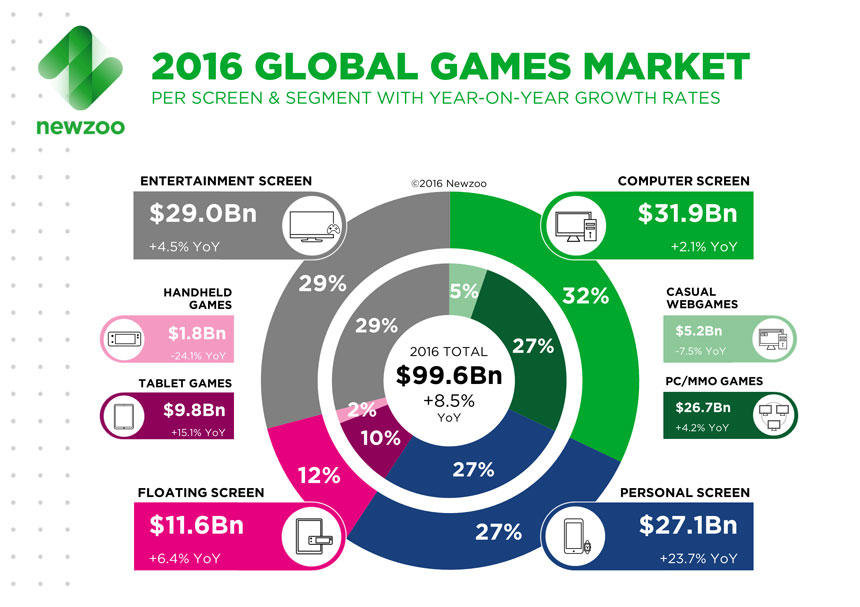
\includegraphics[width=0.6\textwidth]{imagens/1.jpg}
		\caption[Figura ilustrando rendimentos do mercado de jogos no ano de 2016.]{Figura ilustrando rendimentos do mercado de jogos no ano de 2016.}
		\fonte{Adaptado de \citeonline{newzoo}.}
		\label{fig:games}	
	\end{center}
\end{figure}

Porém, enquanto crescem e se tornam uma das aplicações mais populares para a Internet, as trapaças se tornaram um fenômeno chamativo no estado atual dos jogos na \textit{internet}, atuando não só negativamente nas experiências dos outros jogadores como também como um problema de segurança para o jogo e a empresa responsável por ele \cite{trends}. 


Desde sua popularização, a indústria de jogos \textit{online} vem sendo alvo de diferentes tipos de trapaças, que foram evoluindo e modificando-se ao longo dos anos. Muitas delas acabaram causando problemas financeiros para a empresa responsável do jogo. \textit{Age of Empires} e \textit{America’s Army} são alguns exemplos de jogos \textit{online} que sofreram
perdas substanciais devido ao uso de trapaças por seus jogadores \cite{cheatingonlinegames}. 
     
Jogos de \textit{Networked Virtual Environments} (NVEs), reconhecidos pela grande imersão que trazem aos jogadores, seja pela qualidade gráfica ou ambientação de qualidade, acabam sofrendo muito com as trapaças. Como a sensibilidade para perceber atividades ilícitas se torna maior pela ambientação grande deste tipo de jogo, o impacto negativo aos jogadores acaba sendo ainda pior. As trapaças consequentemente tornaram-se uma das formas mais rápidas de destruir a comunidade de um jogo e sua reputação comercial.  

Sabendo do risco e dos problemas de segurança, diversos estudos e trabalhos surgiram para mitigar ou detectar diferentes formas de trapaças que se proliferam com a popularização dos jogos \textit{online} no mercado. Entretanto, assim como alguns tipos de trapaças puderam ser inviabilizadas com boas escolhas de \textit{design} e alterações mínimas, outras formas acabaram necessitando de recursos computacionais altos para serem detectados. Relações de perda e ganho podem ser questionadas pelos criadores do \textit{software}, onde se pode trocar uma maior segurança do jogo por um desempenho e responsividade inferior.


Uma exemplo de vulnerabilidade que pode ser explorada pelos trapaceiros, por exemplo, é a adulteração do \textit{software} que o cliente utiliza no serviço de jogo. Em um modelo cliente-servidor, em que o cliente interage com o servidor, solicitando serviços, e o servidor atende e responde as solicitações, se a mensagem for modificada de forma a tornar-se inválida de acordo com os padrões e regras impostas pelo servidor do jogo, o servidor deve perceber sua ilegitimidade. Caso a ação não seja averiguada no servidor como  inválida, a integridade da partida pode ser comprometida. Trapaças como movimentações ilegais, atributos de personagem acima de seu devido valor, ou mesmo alterações em metadados da partida podem ocorrer devido a este tipo de trapaça. Outras trapaças, como a modificação do \textit{driver} gráfico utilizado para remover as texturas de paredes, são exemplos comuns que podem ser encontrados hoje em dia.


Este trabalho tem como objetivo estudar diferentes comportamentos que podem ser adotados para prevenir ou detectar trapaças em jogos \textit{online}. No Capítulo 2, por existir uma grande variedade de trapaças nos jogos \textit{online}, foram estudados e catalogados os tipos de trapaças existentes em diferentes conjuntos. O trabalho foca em um destes conjuntos de trapaças, abordando estratégias para detectar ou dificultar os tipos de trapaça encontrados neste conjunto. No Capítulo 2.2, os diferentes métodos e estratégias são estudados e analisados, enquanto há um foco maior em dois métodos conhecidos na literatura: uso da execução simbólica para encontrar trapaças, e sistema de auditoria para verificar ações inválidas a partir da definição de estados abstratos e concretos.


O Capítulo 3 apresenta a criação do jogo \textit{online Shooterman}, implementado para este trabalho na linguagem C++, onde se descreve a aplicação tanto do cliente quanto do servidor. Juntamente com o jogo, a implementação das duas estratégias sobre \textit{Shooterman} é demonstrada. No capítulo 4, os resultados obtidos dos dois métodos implementados sobre o jogo \textit{Shooterman} são avaliados e comparados.

\chapter{Trapaças em Jogos Online}
\label{cap:cheating}

Quando se deseja implementar um jogo \textit{online}, onde vários jogadores interagem entre si em um mundo virtual, é importante conhecer os diferentes tipos de trapaças que usuários mal intencionados podem utilizar. Conhecendo as trapaças mais comuns, e as diferentes ferramentas de detecção de trapaças existentes na literatura, torna-se mais fácil de reconhecer quais mecanismos de defesa são recomendados para serem utilizadas em seu jogo.

\section{Definição de Trapaça}

Segundo \cite{yan}, no cenário de jogos \textit{online}, qualquer comportamento que um jogador use para ganhar vantagem sobre outros jogadores ou alcançar um objetivo é considerado trapaça se, de acordo com as regras do jogo ou critério da operadora do jogo (fornecedora de serviços do jogo, que não necessariamente desenvolveu o jogo), a vantagem ou objetivo não deveria ser alcançada. 

A partir da definição de uma trapaça, é possível categorizar os diferentes tipos de trapaças encontrados na literatura, reforçando suas características e consequências negativas aos jogos. Esses diferentes tipos de trapaças abordados pelo trabalho estudado podem ser agrupados em conjuntos que compartilham da mesma fonte do problema. Neste capítulo são abordados os diferentes conjuntos de trapaças existentes, dissertando sobre alguns exemplos e problemas encontrados ao longo da evolução dos jogos \textit{online}. Os conjuntos classificados são divididos em diferentes categorias: adulteração do jogo, abuso das opções do jogo, segurança de rede, engenharia social e exploração da inteligência de máquina.

\subsection{Adulteração do Jogo}
\label{adulteracao}
Neste conjunto, o usuário trapaceiro utiliza tanto do \textit{software} como do \textit{hardware} para obter vantagens sobre os outros usuários. A adulteração do código do jogo e/ou das configurações dos dados da aplicação do cliente, por exemplo, é um tipo de trapaça muito comum em jogos RTS (\textit{Real-Time Stategy}), estilo de jogo onde os jogadores posicionam suas unidades e estruturas para controlar e avançar as áreas do mapa ao mesmo tempo que destroem com a do adversário. Neste cenário, a \textit{Fog of war} (Névoa da Guerra) restringe a visão  do mapa do jogador de acordo com suas tropas e construções, impossibilitando-o de reconhecer o posicionamento inimigo sem ter visão do local que ele se encontra. Com a utilização de um programa de terceiros, é possível filtrar os dados do cliente que informam o posicionamento das tropas adversárias, facilitando o reconhecimento do posicionamento adversário. 

Outro tipo de trapaça, mais comum em jogos FPS (\textit{First Person Shooter}), é o \textit{Wall Hack}. Nos FPS, o jogador controla um personagem que possui acesso à armas de fogo e deve se movimentar pelo cenário, atirando nos adversários e evitando ser atingido. Como o ato de surpreender o adversário e reconhecer seu posicionamento é importantíssimo para este tipo de jogo, qualquer informação sobre o adversário obtida ilegalmente traz uma vantagem imensa para o jogador trapaceiro. Modificar a infraestrutura do cliente com um driver gráfico, por exemplo, pode ser usado para tornar as paredes de um jogo transparentes. No cenário de FPS, isto facilitaria a localização dos outros jogadores, que não seriam capazes de reconhecer o posicionamento do trapaceiro da mesma forma que ele os reconhece.


Modificando o código do jogo, ou utilizando programas de terceiros, é possível modificar mensagens que expressam ações executadas pelos jogadores. Assim, mensagens enviadas pelos clientes podem ser maliciosas ou inválidas de acordo com as regras estabelecidas pelo jogo. Se nestas situações o servidor não perceber a ilegalidade das mensagens, a integridade semântica do jogo pode ser comprometida. Como o custo computacional para verificar todas mensagens de todos clientes é muito alto, algumas estratégias podem ser adotadas para averiguar a integridade das ações dos clientes conectados ao servidor.

Ambos exemplos de trapaças, apesar de utilizarem ferramentas diferentes para conseguir vantagens sobre os adversários, abusam da mesma característica encontrada no lado do cliente: a confiança excessiva que o servidor tem sobre ele. Em todos exemplos, informações relevantes sobre os adversários, como os posicionamentos dos jogadores ou tropas adversárias, situam-se não somente no servidor, mas também no cliente. Estes dados, se descobertos ou alterados, podem gerar benefícios para os jogadores que se aproveitarem desta trapaça.




\subsection{Abuso das Opções do Jogo}

As diversas opções que um jogo disponibiliza podem ser desbalanceadas se executadas em determinada ordem ou de determinada forma, sendo responsabilidade dos desenvolvedores do jogo buscar evitar estes tipos de abusos. Nos exemplos deste conjunto, as trapaças categorizadas comprometem o funcionamento ideal do sistema do jogo, pelo abuso das opções que o jogo dispõe.

O conluio, trapaça em que dois ou mais indivíduos combinam-se para ganharem vantagens desonestas, ocorreu no popular jogo StarCraft \cite{starcraft}, onde dois jogadores arquitetavam uma aliança um com o outro. Cada um perdia uma partida para o outro no modo competitivo, e depois repetiam este processo indefinidamente. Como as derrotas que eles sofriam um do outro não reduziam os pontos de vitória do sistema, apenas as vitórias que obtinham um do outro eram computadas, elevando seus pontos e tornando o processo de subir de posição no jogo muito mais fácil, sem a necessidade de vitórias legítimas. Este tipo de trapaça é conhecido como \textit{"win trading"}.

Outro tipo de trapaça semelhante, conhecido como Abuso dos Procedimentos do Jogo, é o ato de fugir da partida enquanto estiver em uma situação desfavorável. Em alguns jogos, pelo procedimento adotado no sistema, o ato de se desconectar da partida invalida a disputa, independentemente da situação em que ela se encontrava. Caso o sistema não esteja preparado para lidar como este tipo de situação, o jogador que se desconectou não sofre as consequências da derrota da partida, ou seja, se beneficia das falhas derivadas do procedimento adotado.

Alguns serviços de jogos, ou mesmo plataformas, como a plataforma Steam \footnote{http://store.steampowered.com/?l=portuguese}, possibilitam que personagens ou itens virtuais adquiridos nos jogos sejam vendidos por dinheiro real para outros jogadores. Em uma trapaça com espólios virtuais, um usuário trapaceiro pode oferecer um item virtual, receber dinheiro real sobre ele de outro usuário, mas nunca entregar o item como combinado. Além de beneficiar o usuário que utiliza esta trapaça, o prejuízo causado ao alvo é financeiro. 

Em alguns jogos RTS, um jogador trapaceiro pode atrasar seu próprio movimento até saber todos movimentos de seus adversários, ganhando assim uma grande vantagem. Esta forma de \textit{look-ahead} (olhar para a frente) é um tipo de trapaça de tempo \cite{cheat-proof}. Outro trapaça deste tipo é a \textit{suppress-correct}, na qual o jogador obtém vantagens ao enviar propositalmente suas mensagens de \textit{update} nos tempos "certos". 

O uso abusivo de \textit{bugs} ou \textit{loopholes} (falhas no sistema que usuários podem explorar para ganhar uma vantagem injusta ou não intencional), por serem disponibilizados indiretamente,  podem ser categorizados neste conjunto. Os usuários podem usufruir das falhas existentes conhecidas do sistema, sem precisar modificar o código do jogo ou obter dados com outros programas, para se favorecer em relação aos outros jogadores.



\subsection{Segurança de Rede}

Tratando-se dos problemas de segurança de redes tradicionais, pode-se tratar um paralelo com os jogos \textit{online}. O envenenamento de cache DNS, por exemplo, pode ser comparado com um servidor de jogo falso. Se não existe um mecanismo adequado para autenticar o servidor do jogo na aplicação do cliente, um trapaceiro pode coletar vários dados das contas de usuários usuando um servidor falso.

Além do envenenamento de cache DNS, a análise de pacotes pode ser classificada como uma forma de trapaça neste cenário. 
Quando os pacotes da comunicação são trocados em formato de texto, algum usuário trapaceiro pode analisar os pacotes por meio de um analisador de \textit{sniffer} e inserir, deletar ou modificar eventos do jogo ou comandos transmitidos via rede. 

Um trapaceador também pode ganhar vantagens por negar serviços para seus jogadores \textit{peer}. Por exemplo, um jogador pode atrasar as respostas de seu oponente sobrecarregando sua conexão. Outros jogadores \textit{peer} poderiam supor que algo estaria errado com a conexão da vítima, concordando em removê-la da partida. 

\nocite{new}
\nocite{Cadar:2008:KUA:1855741.1855756}
\nocite{Izaiku:2006:CDM:1230040.1230056}
\nocite{Monch:2006:POG:1230040.1230087}
\nocite{Mitterhofer:2009:SBD:1591889.1592174}
\nocite{Yan:2003:SDO:956415.956453}
\nocite{Feng:2008:SMC:1517494.1517497}
\nocite{Kabus:2005:ACD:1103599.1103607}

\subsection {Engenharia Social}

Usuários mal intencionados podem enganar outros usuários, fingindo serem administradores do jogo e requisitando informações pessoais de suas contas. Senhas geralmente são as chaves para grande parte ou todos os dados e autorizações que o usuário tenha no sistema do jogo. Caso sua senha seja comprometida, a vítima pode sofrer consequências como roubo de informações pessoais ou perda de conta.

\subsection{Exploração da Inteligência de Máquina}
Técnicas de inteligência artificial podem ser exploradas por um jogador em alguns jogos online. Por exemplo, o avanço da pesquisa do xadrez na computação produziu diversos programas que podem competir com humanos mestres em diferentes jogos. Em uma partida \textit{online} de xadrez, um usuário trapaceiro pode olhar os melhores candidatos para escolher seu próximo movimento, utilizando um programa de xadrez de computador. Isto se deve ao fato da superioridade, nesta situação específica, da inteligência artificial sobre um ser humano ordinário. Este tipo de trapaça pode existir em diversos outros jogos \textit{online}, incluindo jogos de carta ou jogos de tabuleiro tradicionais, dependendo de suas propriedades do jogo - se o jogo pode ser modelado como um problema computável - e da maturidade de pesquisas de IA deste jogo. Um exemplo recente é a IA do jogo Go \footnote{https://gogameguru.com/what-is-go/}, jogo de tabuleiro de origem chinesa,  que teve sua IA em crescimento nos últimos anos. Em 2002, a IA mais forte de Go podia ser derrotada por um jogador humano amador \cite{go_old}, enquanto que em 2016, a IA criada pela empresa Google \footnote{www.google.com.br} venceu um dos melhores jogadores do mundo no jogo. \cite{ia_google} 

\subsection{Encerramento}

Nesta taxonomia apresentada a cerca das diversas trapaças existentes, o tipo abordado e analisado neste trabalho é focado no conjunto de trapaças representado como adulteração do jogo, mais especificamente sobre o envio de mensagens ilegais ao servidor. As metodologias explanadas no Capítulo \ref{cap:metodologias} trazem algumas soluções para a resolução destes problemas onde o cliente deliberadamente modifica sua versão do jogo ou suas mensagens na comunicação, podendo realizar ações fora das regras estabelecidas previamente.


\section{Métodos contra Trapaças em Jogos Online}
\label{cap:metodologias}

Diferentes métodos podem ser empregados para evitar ou detectar trapaças que usuários mal intencionados estejam utilizando. Focando em um conjunto mais restrito de trapaças, mais especificamente, as apresentados no Capítulo \ref{adulteracao}, diferentes estratégias podem ser abordadas para se prevenir. Dois destes métodos, abordados em estudos anteriores por \cite{NVE} e \cite{implementacaosimbolica}, são explicados nos Capítulos \ref{simbolics} e \ref{semantics}, e implementados nos Capítulos \ref{implementsimbolic} e \ref{implementsemantic}.

\subsection{Verificação do Executável}
É notório que uma das formas de executar trapaças é alterar o executável do jogo, modificando dados de atributos do personagem, ou permitindo que determinadas ações inicialmente proibidas sejam possíveis de serem executadas. 
Uma das formas de evitar isso é checar periodicamente a conformidade do executável do usuário. Por exemplo, o cliente do jogo, antes de possibilitar que o usuário se conecte ao jogo com sua conta, utiliza um verificador no executável do usuário e o compara com um executável válido. Uma estratégia é a utilização de uma \textit{hash} criptográfica, que permite a compressão unidirecional (compressão que não pode ser revertida) do executável do cliente, que é então enviado ao servidor e comparada com a \textit{hash} previamente criada de um executável confiável. Se forem compatíveis, conclui-se que o usuário não alterou seu cliente de jogo. Esta estratégia, entretanto, ainda não resolve outros problemas encontrados em um cliente sem autoridade. Outros programas de terceiros ainda podem interagir com as informações que se encontram na aplicação, possibilitando que ações inválidas ocorram se o servidor não averiguá-las. 


\subsection{Cliente sem autoridade sobre o estado do servidor}
A estratégia adotada mais comum para se prevenir de maus comportamentos dos clientes é garantir que o cliente não possua estado de autoridade que possa afetar o servidor ou a aplicação. O básico dessa abordagem é enviar ao servidor todas entradas do cliente, que são executados e validados diretamente no servidor. Esta estratégia não se preocupa com o processamento extensivo realizado no servidor, afinal, nenhum processamento crítico é executado no computador do cliente. Pode-se categorizar este tipo de estratégia como inviável para aplicações com custos computacionais significativos ou com público alvo grande, o que é o caso para a maioria dos jogos \textit{online} encontrados atualmente. Para jogos onde o tempo de resposta não é impactante na experiência proporcionada aos jogadores, como em jogos de turnos de estratégia, esta opção pode ser considerada viável. Jogos de xadrez \textit{online} ou jogos de cartas, por exemplo, são estilos de jogos que não são afetados tão negativamente pelo tempo de resposta maior do servidor. 

\subsection{Validação por outro cliente}

O servidor pode agir como o meio de comunicação entre dois clientes, fazendo com que outro jogador valide a mensagem enviada. Nesta estratégia, a validação ocorre diretamente na aplicação de outro usuário que retorna ao servidor se a ação é considerada válida ou não. Apesar do custo computacional acontecer diretamente no cliente, e na maioria dos casos, esse processamento ser insignificante isoladamente e rápido, o número de mensagens de uma ação é dobrada. Para cada mensagem enviada do cliente ao servidor, outras duas novas mensagens devem ser transmitidas, do servidor ao cliente dois, e novamente do cliente dois ao cliente um. Outro problema é a divulgação de informações que o jogador poderia não ter acesso. Em uma situação onde o cliente 2 recebe informações do cliente 1 para validar, ele acaba ganhando acesso aos dados a serem verificados. Em cenários onde existem informações confidenciais a outros jogadores, esta estratégia não é muito útil, pela necessidade da quebra de confidenciabilidade sobre os dados a serem verificados.


\subsection{Validação com Execução Simbólica}

\label{simbolics}

A execução simbólica é uma das formas de analisar um programa e determinar quais entradas dele causaram a execução de cada parte do programa. Em vez de utilizar valores de entrada concretos, como números inteiros ou de ponte flutuante, os valores são transformados em valores simbólicos, e, como eles, sua saída é gerada simbolicamente. Seu uso mais convencional é no teste de \textit{software}, utilizado na análise de erros. Nessa análise, as entradas e condições que acarretaram a ocorrência dos erros são previstas utilizando a execução simbólica. 

A execução simbólica utiliza o paradigma Programação com Restrições, que consiste em especificar quais critérios (definidos formalmente como restrições) uma solução deve cumprir. Um resolvedor de restrições então utilizará as restrições especificadas juntamente com o fluxo lógico do programa para descobrir quais valores concretos de entrada gatilharam a ocorrência dos erros.

A Figura \ref{fig:exsimb} representa o fluxograma gerado após a execução simbólica de \textit{x}. No exemplo, verifica-se se \textit{x} é maior que zero, e depois, se \textit{x} é maior que dez. No primeiro teste, dois fluxos de execução podem acontecer: ou \textit{x} é maior que zero, ou não. Em cada um destes novos fluxos de execução, é verificado se \textit{x} é maior que dez. No segundo fluxo, a hipótese de \textit{x} ser maior que dez é descartada, afinal, \textit{x} mostrou-se menor que zero no teste anterior.  

\begin{figure}
	\begin{center}
		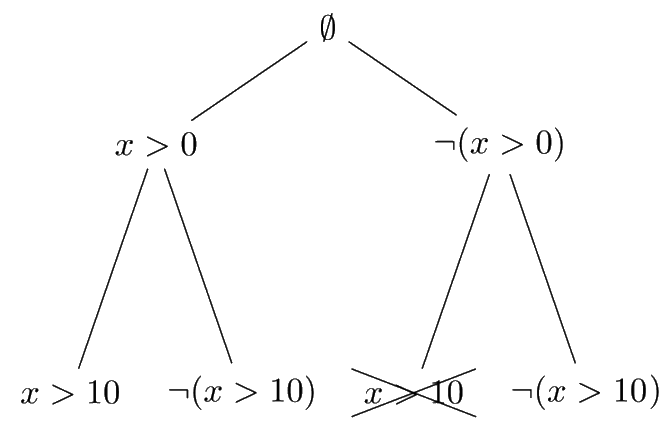
\includegraphics[width=0.6\textwidth]{imagens/exemplosimbolic.png}
		
		\caption[Exemplo de execução simbólica de um programa simples.]{Exemplo de execução simbólica de um programa simples.}
		\fonte{Retirado da apresentação de \citeonline{tixinha}.}
		\label{fig:exsimb}	
	\end{center}

\end{figure}


 \cite{implementacaosimbolica} demonstra um exemplo prático de uma implementação simbólica em um jogo simples.


\begin{figure}[h!]
		\small
		\begin{multicols}{2}

		100: \textit{loc} $\leftarrow$ 0; \\
		101: \\
		102: enquanto true faça \\
		103:\tab    key $\leftarrow$ lekey(); \\
		104:\tab	se key = ESC entao \\
		105:\tab\tab		fimjogo(); \\
		106:\tab	senao se key = '$\uparrow$' entao \\
		107:\tab\tab		loc $\leftarrow$  loc + 1; \\
		108:\tab	senao se key = '$\downarrow$' entao \\
		109:\tab\tab		loc $\leftarrow$  loc -- 1; \\
		110:\tab	fim se \\
		111:\tab envialocalizacao(loc); \\
		112: fim enquanto \\

		\footnotesize
		\textit{(a) Exemplo simples de um cliente}

		\small
		200: \textit{loc\_ant} $\leftarrow$ 0; \\
		201: \textit{loc} $\leftarrow$ \textit{loc\_ant}; \\
		202: enquanto true faça \\
		203:\tab	key $\leftarrow$ simbolico; \\
		204:\tab	se key = ESC entao \\
		205:\tab\tab		fimjogo(); \\
		206:\tab	senao se key = '$\uparrow$' entao \\
		207:\tab\tab		loc $\leftarrow$  loc + 1; \\
		208:\tab	senao se key = '$\downarrow$' entao \\
		209:\tab\tab		loc $\leftarrow$  loc -- 1; \\
		210:\tab	fim se \\
		211:\tab	\textit{breakpoint}; \\
		212: fim enquanto \\ 

		\footnotesize
		\textit{(b) Exemplo instrumentado para executar simbolicamente}

		\end{multicols}

	\caption[Exemplo de execução simbólica com código.]{Exemplo de execução simbólica com código.}
	\fonte{Adaptado de \citeonline{implementacaosimbolica}.}
	\label{fig:codigo1}	

\end{figure}


Neste exemplo simples do jogo Pong da Figura \ref{fig:codigo1}, a aplicação do cliente lê a todo instante as teclas pressionadas pelo usuário, atualizando a posição do jogador de acordo com a direção em que a tecla está pressionada. Em cada iteração do laço principal do programa, o servidor também é atualizado, recebendo a posição atual em que o cliente se encontra. 

Já na versão simbólica do programa, a nova variável \textit{loc\_ant} é instanciada como uma variável simbólica, assim como a variável existente \textit{key}. Um \textit{breakpoint} é criado substituindo a função \textit{envialocalização}, possibilitando que sempre que o fluxo do programa alcançá-lo, se obtenha as restrições geradas em todas variáveis simbólicas. Percebe-se que o envio da mensagem ao servidor não ocorre na versão simbólica, afinal, ela não visa ser uma versão executável tradicional da aplicação, mas sim uma versão que simula os fluxos de operações realizadas durante uma execução.

Para cada escolha gerada na execução do programa, um novo ramo de execução é criado juntamente com uma nova restrição. Essas escolhas são criadas no laço principal, em cada uma de suas iterações. Consequentemente, é possível construir um conjunto de restrições, que representa quais possíveis restrições podem ser geradas em cada iteração do laço principal. 
A partir do exemplo da Figura \ref{fig:codigo1}, dada a iteração \textit{j}, define-se que o conjunto de possíveis restrições que podem ocorrer nessa iteração $C_j$ é o conjunto

\textit{(loc = loc\_ant + 1) $\vee$  (loc = loc\_ant -- 1) $\vee$ (loc = loc\_ant) } \\

Como pode ser deduzido, cada elemento do conjunto $C_j$ depende dos valores anteriores atribuídos a variável \textit{loc\_ant}. Considerando um cenário onde o servidor sabe a última posição do cliente, por exemplo, três possíveis restrições podem ser verificadas na próxima mensagem que o cliente enviar. Caso nenhuma dessas restrições for atendida, ou seja, a variável recebida não for igual, um a mais ou um a menos que o valor anterior, é dedutível que a mensagem enviada pelo cliente é falsa e ele está trapaceando.


\subsection{Protocolo de Integridade de Semântica Segura}
\label{semantics}

Esta abordagem utiliza um procedimento de auditoria, que é executado por um Servidor de Auditoria. Sua estratégia utiliza o conceito de estados abstratos e concretos na troca de mensagens entre as ações de um cliente. A partir dos estados dos clientes, é utilizado um algoritmo para verificar a integridade da sequência destes estados com a utilização de processos de auditoria.

\subsubsection {Definição de Estados}
\label{cap:definicaoestado}

Este método utiliza o conceito de estados abstratos e concretos, que são ilustrados na Figura \ref{fig:abstracao}. No exemplo que a Figura \ref{fig:abstracao} traz, duas aproximações foram pensadas para checar se em um determinado vetor \textit{a}, a posição \textit{i} do vetor, \textit{a[i]}, excede os limites do vetor. No primeiro modelo criado, existe um conjunto com todos possíveis valores que \textit{i} pode conter, enquanto que, no segundo modelo, existem possíveis intervalos de valores possíveis que podem conter \textit{i}. Nesta representação simples, é preferível utilizar o segundo modelo, pela sua maior abstração dos valores que \textit{i} pode obter. A primeira aproximação utiliza valores concretos para a resolução do problema, enquanto a segunda utiliza valores abstratos. As setas verdes da figura representam as funções de transformação de domínio que ocorrem de um modelo para o outro.  A transformação $\delta$ representa uma função de abstração (transposição do domínio mais concreto para o mais abstrato), e $\gamma$ representa o processo inverso, uma função de concretização (transposição do domínio mais abstrato para o concreto).

\begin{figure}[h!]
	\begin{center}
		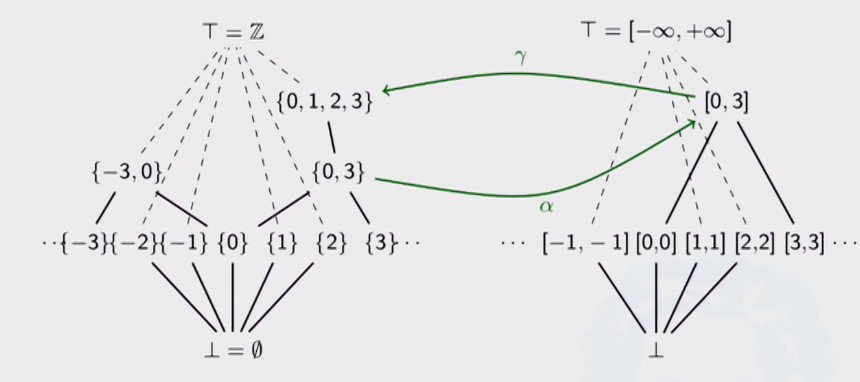
\includegraphics[width=0.6\textwidth]{imagens/abstracao.png}
		\caption[Exemplo da função de Abstração e Concretização]{Exemplo da função de Abstração e Concretização.}
		\fonte{Retirado da apresentação de \citeonline{galoi}.}
		\label{fig:abstracao}
	\end{center}
\end{figure}

Formalmente, define-se que a partir de um estado abstrato \textit{s}, $\gamma$ (s) representa o conjunto de possíveis concretizações que podem ocorrer a \textit{s}. Já um estado concreto S, sua função $\delta$(S) corresponde a um único estado abstrato. Em outras palavras, um estado abstrato pode representar diferentes estados concretos, enquanto que um estado concreto representa um único estado abstrato. Alterações de um estado ocorrem constantemente, e são representadas por $\Delta$, ou \textit{diff}, sendo ele a mudança sofrida de um estado para outro. Em outras palavras, o estado S atualizado para o estado S' sofre a diferença $\Delta$, portanto, S' $=$ S + $\Delta$. 

As funções de transformação de domínio $\gamma$ e $\delta$ podem ser aplicadas não somente nos estados, mas também nas diferenças entre estados. $\gamma$($\delta$), por exemplo, expressa a abstração de uma \textit{diff} $\delta$ qualquer, enquanto $\delta$ representa a concretização da \textit{diff} $\delta$. Algumas conclusões podem ser estabelecidas sobre as \textit{diff}, como $\gamma$(S') $=$ $\gamma$(S) + $\gamma$($\delta$) se S'$=$ S + $\Delta$. Sendo $\alpha$ a representação de uma abstração de uma \textit{diff} $\Delta$ aplicada ao estado S, pode-se deduzir que $\Delta$ $\in$ $\gamma$(S, $\alpha$($\Delta$)) e para cada $\Delta$´ $\in$ $\gamma$(S, $\alpha$($\Delta$)) obtém-se $\alpha$(S $+$ $\Delta$´) $=$ $\alpha$(S´).


\subsubsection{Aplicação dos estados}

No Protocolo de Integridade de Semântica Segura (SSIP), representam-se as informações do servidor e do cliente em estados, que podem ser tanto abstratos quanto concretos. A representatividade destes estados pode ser encontrada na implementação realizada, referenciada no Capítulo \ref{cap:desenvolvimento}. 

Neste protocolo, o servidor principal da aplicação é denominado Servidor de Estados, que equivale a um servidor convencional de uma NVE, implementado para interagir com os usuários e estabelecer comunicações e trocas de dados sobre as informações do jogo. O servidor de estados contém um estado central abstrato ASTATE, que contém informações relevantes de todos clientes. Imaginando o estado ASTATE como um vetor, por exemplo, cada uma de suas partes é relevante para um cliente conectado a ele. Em outras palavras, de todo estado ASTATE, apenas a parcela ASTATE[$cli_i$] é relevante para o cliente $cli_i$.

Como os clientes possuem estados concretos das informações do jogo, e o servidor possui apenas uma versão abstrata disso,
as funções de transposição de domínios apresentadas no capítulo \ref{cap:definicaoestado} acabam ocorrendo constantemente na comunicação cliente-servidor. Exceto na primeira mensagem de inicialização do cliente com o servidor, por exemplo, todas mensagens posteriores enviadas pelo cliente passam pela função de transposição de abstração. Estas abstrações das mensagens do cliente existem para amenizar o excesso de processamento gerado no servidor nos testes que executa para verificar a validade da mensagem. 

Um exemplo simplificado deste caso encontra-se no jogo implementado \textit{Shooterman} (capítulo \ref{shoterman}). Enquanto variáveis como posição são mantidas no servidor, variáveis de controle mais refinado das ações do personagem são mantidas unicamente no cliente de jogo, como por exemplo, o tempo de recarga de suas ações. Essas informações do estado do jogador são mais abstraídas para o servidor, enquanto são concretas para o cliente do jogador.

Em cada um dos ciclos do cliente, ele envia ao servidor uma abstração $\gamma$ $=$ $\alpha$($\Delta$), que contém uma abstração da \textit{diff} dos últimos estados. Esta abstração é denominada \textit{diff de requisição}. Após o recebimento da \textit{diff} de requisição, o servidor valida a mensagem de acordo com suas semânticas pré-estabelecidas e retorna ao cliente uma confirmação das mudanças requisitadas e das atualizações realizadas pelos outros clientes conectados a NVE. 

Utilizando esta técnica, um cliente malicioso ainda pode violar as regras semânticas estabelecidas pelo servidor, pela susceptibilidade do protocolo, afinal ele só pode verificar se as atualizações abstratas são consistentes com o estado abstrato, sem levar em consideração os valores concretos avaliados. Para solucionar esta falha, ciclos de auditoria são utilizados constantemente para verificar as atualizações de acordo com os estados concretos dos clientes conectados.

\subsubsection{SSIP}
Outro servidor, denominado Servidor de Auditoria, é utilizado para verificar a integridade semântica dos estados que são constantemente atualizados pelos clientes. Este servidor requisita a um cliente sua sequência de atualizações de estados concretos de um tempo específico junto com seu estado concreto inicial completo, e a partir deles, computa os estados em ordem, verificando sua integridade.

Uma série de operações devem ser seguidas na comunicação do cliente com o servidor de auditoria, e \cite{NVE} dividiu estas operações em três diferentes protocolos, que são apresentados a seguir. Nas ilustrações dos protocolos, são utilizados as setas $\rightarrow$ que representam pacotes enviados de forma não-confiável, e as setas $\hookrightarrow$, que representam pacotes enviados de forma confiável.

\subsubsection{Protocolo de Inicialização}
\label{protocoloinicializacao}

Este protocolo ocorre quando o cliente inicia seu contato com o servidor. A Figura 2.2 mostra a sequência de passos que deve ser tomada no início da comunicação do cliente com o servidor do jogo.

\begin{figure}[h!]
	\begin{center}
		\fbox{\begin{minipage}{30em}
		\begin{enumerate}
		\small
		\item cli inicializa \textit{t} $:=$ 0 e envia requisição de solicitação ao servidor de estado
		\item Servidor de estado $\rightarrow$ servidor de auditoria : \textit{k} $:=$ GeraMac($1^{n}$)
		\item Servidor de auditoria $\rightarrow$ cli : \textit{h} $:=$ GeraHash($1^{n}$)
		\item Servidor de estado escolhe o estado S do conjunto ASTATE 
		\item Servidor de estado $\rightarrow$ cli: AuthMsg(\textit{k}, S $\parallel$ $n_0$, cli)
		\item cli define $S_0$ como S.
		\item cli $\hookrightarrow$ servidor de auditoria: $Q_0$ $:=$ $CFHash_h$($S_0$)
		\end{enumerate}

		\end{minipage}}

	\end{center}
	\fonte{Traduzido de \cite{NVE}. Protocolo Initialize}
	\caption[Definição do Protocolo de Inicialização.]{Definição do Protocolo de Inicialização.}
	\label{fig:inicializar}	
	
\end{figure}

Primeiramente, o cliente inicializa a variável \textit{t}, que representa o número do ciclo em que ele se encontra. No passo 2, o servidor de estado envia ao servidor de auditoria a variável \textit{k}, que representa uma chave criptográfica. Essa chave criptográfica é gerada usando o \textit{Message Authentication Code} (MAC), algoritmo que recebe como entrada uma chave secreta e uma mensagem a ser autenticada, gerando uma MAC, ou etiqueta\cite{Krawczyk:1997:HKM:RFC2104}.

No terceiro passo, define-se \textit{h}, índice que representará qual função \textit{hash} o cliente utilizará posteriormente em suas mensagens enviadas a auditoria. O parâmetro \textit{n} da função GeraHash representa o nível de segurança da \textit{hash}. 

Em seguida, o servidor envia uma mensagem ao cliente contendo o estado S escolhido no quarto passo, e o cliente a define como seu estado primário $S_0$. A mensagem é enviada junto com a etiqueta MAC gerada.

No começo de cada auditoria, o cliente envia ao servidor de auditoria uma \textit{hash} de seu estado concreto completo. Apesar do custo computacional ser relativamente alto, dependendo do tamanho da informação contida em um estado concreto, a mensagem precisa chegar entre os próximos \textit{n} ciclos do cliente. O último passo deste protocolo demonstra o envio do estado concreto $S_0$ ao servidor de auditoria. Após o envio, a inicialização é finalizada.


\subsubsection{Procotolo de Atualização dos Status}

Este protocolo é executado em cada ciclo do cliente. Ele consiste na atualização do estado do cliente após a confirmação do servidor, conforme a Figura \ref{fig:atualizacao} ilustra. Cada ciclo de cliente ocorre em cada instante de tempo que o cliente pode interagir com o jogo. Geralmente, pode-se definir que um ciclo ocorre a cada frame de execução do jogo.

Além de manter seu estado concreto atual, o cliente mantém seus estados anteriores em um \textit{buffer} local, contendo até três estados completos e 3\textit{n} \textit{diffs} geradas ao longo de sua execução. Enquanto novos estados e suas \textit{diffs} são inseridas no \textit{buffer}, seus conteúdos antigos podem ser removidos por não serem mais úteis no protocolo. Essas características do \textit{buffer} correspondem a um processo semelhante ao de uma janela deslizante, onde as informações relevantes que o \textit{buffer} armazena são sempre as mais recentes. Todas mensagens recebidas do servidor de auditoria também são armazenadas no cliente de acordo com o intervalo de tempo determinado pela janela deslizante de seu \textit{buffer}.

\begin{figure}[h!]
	\begin{center}
		\fbox{\begin{minipage}{30em}
		\begin{enumerate}
		\small
		\item cli computa a mudança $\Delta_{\textit{t}+1}$ e gera uma nova abstração $\delta_{\textit{t}+1}$ 
		\item cli $\rightarrow$ servidor de estado$:$ $\delta_{\textit{t}+1}$
		\item Servidor de estado computa a atualização $\delta '_{\textit{t}+1}$ e atualiza ASTATE
		\item Servidor de estado $\rightarrow$ cli$:$ $M_{\textit{t}+1}$ $:=$ AuthMsg(\textit{k}, $\delta_{t+1}$ $\parallel$ 
		$\textit{n}_t$ + 1, cli)
		\item cli armazena $\Delta_{\textit{t}+1}$ e computa $S_{t+1}$ $=$ $S_t$ $+$ $\Delta '_{t+1}$
		\item cli $\hookrightarrow$ servidor de auditoria $:$ $D_{t+1}$ $:=$ $Hash_h$($\Delta '_{t+1}$)
		\item cli incrementa variável \textit{t}
		\item caso \textit{t} mod \textit{l} $=$ 0
			\begin{enumerate}
				\small
				\item cli deleta todos \textit{diffs} $\Delta '_{t-i}$
				\item cli armazena $S_t$ e começa a computar $Q_t$ $:=$ $Hash_h$ ($S_t$)
			\end{enumerate}

		\end{enumerate}

		\end{minipage}}
		\fonte{Traduzido de \cite{NVE}. Protocolo StatusUpdate}
		\caption[Definição do Protocolo de Atualização dos Status.]{Definição do Protocolo de Atualização dos Status.}
		\label{fig:atualizacao}
	\end{center}

		
\end{figure}

No início de cada atualização, o cliente gera a mudança $\Delta$ de acordo com sua ação, gerando uma abstração $\delta$ que é então enviada ao servidor de estado. Ele computa esta atualização a partir da abstração recebida, atualizando seu ASTATE. Após isso, ele envia uma mensagem de confirmação ao cliente com sua etiqueta MAC para identificar sua autenticidade como servidor.

Confirmada a mudança $\Delta$ gerada pelo cliente, ele atualiza seu novo estado, agora sendo $S_{t+1}$, como o passo 5 representa. A partir do tipo de \textit{hash} definido no protocolo anterior de atualização realizado anteriormente declarado na variável \textit{h}, o cliente gera um \textit{hash} dessa mudança $\Delta$ e envia ao servidor de auditoria. O cliente incrementa o número de ciclos armazenado em \textit{t}, e verifica se \textit{t} é múltiplo de \textit{l}. Se for, ele remove todas \textit{diffs} mais antigas geradas anteriormente, além de armazenar seu estado concreto, computar a \textit{hash} deste estado, e enviá-la ao servidor de auditoria.

\subsubsection{Procotolo de Auditoria}
\label{protocoloAuditoria}

É no protocolo de auditoria que se verifica a validade de um cliente em um certo período de tempo onde ele envia suas mensagens. O primeiro passo, como observado na Figura \ref{fig:auditoria}, é enviar uma mensagem ao cliente convocando-o a uma auditoria, juntamente com o índice $t_0$ que representará o índice inicial das ações que serão enviadas.

\begin{figure}[h!]
	\begin{center}
		\fbox{
			\begin{minipage}{30em}
			\begin{enumerate}
			\small
			\item Servidor de auditoria $\rightarrow$ cli $:$  \textit{audit} $\parallel$ $t_0$
			\item cli computa $t_a$ $=$ $\lfloor$ $\frac{t_0}{l}$ $-$ 2 $\rfloor$ \textit{l}
			\item cli $\rightarrow$ servidor de auditoria $:$ $S_{t_a}$ $\parallel$ $\Delta '_{t_a}$ + 1 $\parallel$ ... $\parallel$ $\Delta '_{t_o}$ $\parallel$ $M_{t_a}$ + 1 $\parallel$ ... $\parallel$ $M_{t_0}$


			\item Para \textit{i} $=$ $\textit{t}_a$, ... $\textit{t}_0$ $-$ 1 onde $\hat{S}_{t_a}$ $=$ $S_{t_a}$
				o servidor de auditoria computa	$\hat{S}_{i+1}$ $=$ $\hat{S}_i$ $+$ $\Delta '_{i+1}$ 

			\item Para todo \textit{i} $=$ $t_a$ $+$, ..., $t_0$ o servidor de auditoria determina se $\Delta '_i$ está de acordo com as regras estipuladas

			\item Para todo \textit{i} $=$ $t_a$ $+$, ..., $t_0$, o servidor de auditoria verifica o MAC e a Hash enviadas pelo cli.

			\item Servidor de auditoria compara as \textit{hashs} $S_{t_a}$ com $Q_{t_a}$ e $\hat{S}_{t_a}$ + l com $Q_{t_a}$ + l.
			\end{enumerate}

			\end{minipage}
		}

	\caption[Definição do Protocolo de Auditoria.]{Definição do Protocolo de Auditoria.}

	\fonte{Traduzido de \cite{NVE}. Protocolo Audit} 
	\label{fig:auditoria}
	
	\end{center}
\end{figure}

Quando ciente da abertura da auditoria, o cliente computa $t_a$. Este valor representa o índice do ciclo mais recente que ele começará a enviar. Então o cliente envia as \textit{diffs} das mensagens de $t_a$ até $t_0$. Em outras palavras, todas mudanças que ocorreram em seu estado deste o instante $t_0$ (início da auditoria) até o instante $t_a$ (representado pela fórmula do passo 2) são enviadas ao servidor de auditoria. Além das \textit{diffs}, seu estato concreto também é enviado, juntamente com todas mensagens $M_i$ no mesmo intervalo de \textit{a} a \textit{0}. Estas mensagens são as mensagens de confirmação recebidas pelo servidor de estado no protocolo de Atualização dos Status (vide Figura 3.3, passo 4).

Em um exemplo, supondo que \textit{l} seja 10, ou seja, a cada 10 ciclos do cliente, uma nova \textit{hash} do estado concreto é gerada e enviada ao servidor de auditoria. Na abertura da auditoria, o servidor de auditoria envia ao cliente $t_0$ equivalente a 30. A partir disso, o cliente calcula $t_a$, como no passo 2, resolvendo que $t_a$ = 10. O cliente então envia seu estado concreto do ciclo $t_a$, juntamente com todas \textit{diffs} do ciclo 10 ao 30, e todas mensagens de confirmação M do ciclo 10 ao 30. O servidor de auditoria então descobre todos estados concretos do ciclo 10 ao 30, usando as abstrações recebidas (passo 4). O servidor também verifica se as \textit{diffs} são consistentes com as abstrações $\delta '$(passo 5).

Com isso, usando as mensagens recebidas anteriormente $Q_i$ (vide Figura \ref{fig:inicializar}, passo 7), e $D_i$ (Figura \ref{fig:atualizacao}, passo 6), o servidor de auditoria consegue comparar as abstrações recebidas aplicando-as a $Q_i$ e verificar se equivalem as ações concretas $D_i$. Depois, ele verifica tanto o MAC contido nas mensagens $M_i$ com \textit{i} variando de $t_a$ a $t_i$, quanto as \textit{hashs} das \textit{diffs} $\Delta '$ com as textit{hashs} recebidas anteriormente em D. Depois o servidor de auditoria compara as \textit{hash} dos estados concretos inicial e final recebidas com os estados gerados atráves do passo 4 e transformados em \textit{hash} para esta comparação.
%\chapter{Métodos contra Trapaças em Jogos Online}
\label{cap:metodologias}

Diferentes métodos podem ser empregados para evitar ou detectar trapaças que usuários mal intencionados estejam utilizando. Focando em um conjunto mais restrito de trapaças, mais especificamente, as apresentados no Capítulo \ref{adulteracao}, diferentes estratégias podem ser abordadas para se prevenir. Dois destes métodos, abordados em estudos anteriores por \cite{NVE} e \cite{implementacaosimbolica}, são explicados nos Capítulos \ref{simbolics} e \ref{semantics}, e implementados nos Capítulos \ref{implementsimbolic} e \ref{implementsemantic}.

\section{Verificação do Executável}
É notório que uma das formas de executar trapaças é alterar o executável do jogo, modificando dados de atributos do personagem, ou permitindo que determinadas ações inicialmente proibidas sejam possíveis de serem executadas. 
Uma das formas de evitar isso é checar periodicamente a conformidade do executável do usuário. Por exemplo, o cliente do jogo, antes de possibilitar que o usuário se conecte ao jogo com sua conta, utiliza um verificador no executável do usuário e o compara com um executável válido. Uma estratégia é a utilização de uma \textit{hash} criptográfica, que permite a compressão unidirecional (compressão que não pode ser revertida) do executável do cliente, que é então enviado ao servidor e comparada com a \textit{hash} previamente criada de um executável confiável. Se forem compatíveis, conclui-se que o usuário não alterou seu cliente de jogo. Esta estratégia, entretanto, ainda não resolve outros problemas encontrados em um cliente sem autoridade. Outros programas de terceiros ainda podem interagir com as informações que se encontram na aplicação, possibilitando que ações inválidas ocorram se o servidor não averiguá-las. 


\section{Cliente sem autoridade sobre o estado do servidor}
A estratégia adotada mais comum para se prevenir de maus comportamentos dos clientes é garantir que o cliente não possua estado de autoridade que possa afetar o servidor ou a aplicação. O básico dessa abordagem é enviar ao servidor todos \textit{inputs} do cliente, que são executados e validados diretamente no servidor. Esta estratégia não se preocupa com o processamento extensivo realizado no servidor, afinal, nenhum processamento crítico é executado no computador do cliente. Pode-se categorizar este tipo de estratégia como inviável para aplicações com custos computacionais significativos ou com público alvo grande, o que é o caso para a maioria dos jogos \textit{online} encontrados atualmente. Para jogos onde o tempo de resposta não é impactante na experiência proporcionada aos jogadores, como em jogos de turnos de estratégia, esta opção pode ser considerada viável. Jogos de xadrez \textit{online} ou jogos de cartas, por exemplo, são estilos de jogos que não são afetados tão negativamente pelo tempo de resposta maior do servidor. 

\section{Validação por outro cliente}

O servidor pode agir como o meio de comunicação entre dois clientes, fazendo com que outro jogador valide a mensagem enviada. Nesta estratégia, a validação ocorre diretamente na aplicação de outro usuário que retorna ao servidor se a ação é considerada válida ou não. Apesar do custo computacional acontecer diretamente no cliente, e na maioria dos casos, esse processamento ser insignificante isoladamente e rápido, o número de mensagens de uma ação é dobrada. Para cada mensagem enviada do cliente ao servidor, outras duas novas mensagens devem ser transmitidas, do servidor ao cliente dois, e novamente do cliente dois ao cliente um. Outro problema é a divulgação de informações que o jogador poderia não ter acesso. Em uma situação onde o cliente 2 recebe informações do cliente 1 para validar, ele acaba ganhando acesso aos dados a serem verificados. Em cenários onde existem informações confidenciais a outros jogadores, esta estratégia não é muito útil, pela necessidade da quebra de confidenciabilidade sobre os dados a serem verificados.


\section{Validação com Execução Simbólica}

\label{simbolics}

A execução simbólica é uma das formas de analisar um programa e determinar quais entradas dele causaram a execução de cada parte do programa. Em vez de utilizar valores de entrada concretos, como números inteiros ou de ponte flutuante, os valores são transformados em valores simbólicos, e, como eles, sua saída é gerada simbolicamente. Seu uso mais convencional é no teste de \textit{software}, utilizado na análise de erros. Nessa análise, as entradas e condições que acarretaram a ocorrência dos erros são previstas utilizando a execução simbólica. 

A execução simbólica utiliza o paradigma Programação com Restrições, que consiste em especificar quais critérios (definidos formalmente como restrições) uma solução deve cumprir. Um resolvedor de restrições então utilizará as restrições especificadas juntamente com o fluxo lógico do programa para descobrir quais valores concretos de entrada gatilharam a ocorrência dos erros.

A Ilustração \ref{fig:exsimb} representa o fluxograma gerado após a execução simbólica de \textit{x}. No exemplo, verifica-se se \textit{x} é maior que zero, e depois, se \textit{x} é maior que dez. No primeiro teste, dois fluxos de execução podem acontecer: ou \textit{x} é maior que zero, ou não. Em cada um destes novos fluxos de execução, é verificado se \textit{x} é maior que dez. No segundo fluxo, a hipótese de \textit{x} ser maior que dez é descartada, afinal, \textit{x} mostrou-se menor que zero no teste anterior.  

\begin{ilustracao}
	\begin{center}
		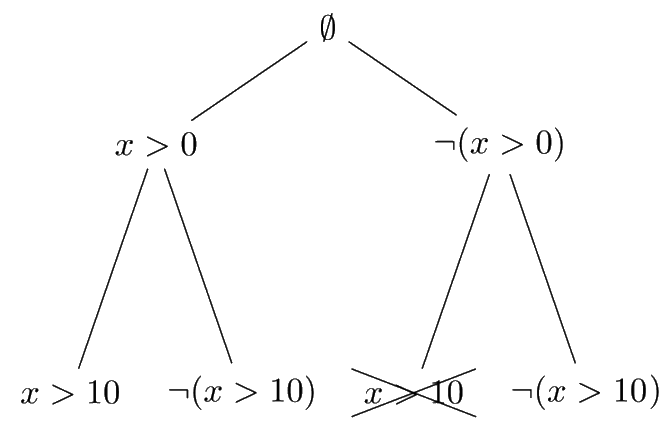
\includegraphics[width=0.6\textwidth]{imagens/exemplosimbolic.png}
		
		\caption[Exemplo de execução simbólica de um programa simples.]{Exemplo de execução simbólica de um programa simples.}
		\fonte{Retirado da apresentação de \citeonline{tixinha}.}
		\label{fig:exsimb}	
	\end{center}

\end{ilustracao}


 \cite{implementacaosimbolica} demonstra um exemplo prático de uma implementação simbólica em um jogo simples.


\begin{figure}[h!]
		\small
		\begin{multicols}{2}

		100: \textit{loc} $\leftarrow$ 0; \\
		101: \\
		102: enquanto true faça \\
		103:\tab    key $\leftarrow$ lekey(); \\
		104:\tab	se key = ESC entao \\
		105:\tab\tab		fimjogo(); \\
		106:\tab	senao se key = '$\uparrow$' entao \\
		107:\tab\tab		loc $\leftarrow$  loc + 1; \\
		108:\tab	senao se key = '$\downarrow$' entao \\
		109:\tab\tab		loc $\leftarrow$  loc -- 1; \\
		110:\tab	fim se \\
		111:\tab envialocalizacao(loc); \\
		112: fim enquanto \\

		\footnotesize
		\textit{(a) Exemplo simples de um cliente}

		\small
		200: \textit{loc\_ant} $\leftarrow$ 0; \\
		201: \textit{loc} $\leftarrow$ \textit{loc\_ant}; \\
		202: enquanto true faça \\
		203:\tab	key $\leftarrow$ simbolico; \\
		204:\tab	se key = ESC entao \\
		205:\tab\tab		fimjogo(); \\
		206:\tab	senao se key = '$\uparrow$' entao \\
		207:\tab\tab		loc $\leftarrow$  loc + 1; \\
		208:\tab	senao se key = '$\downarrow$' entao \\
		209:\tab\tab		loc $\leftarrow$  loc -- 1; \\
		210:\tab	fim se \\
		211:\tab	\textit{breakpoint}; \\
		212: fim enquanto \\ 

		\footnotesize
		\textit{(b) Exemplo instrumentado para executar simbolicamente}

		\end{multicols}

	\caption[Exemplo de execução simbólica com código.]{Exemplo de execução simbólica com código.}
	\fonte{Adaptado de \citeonline{implementacaosimbolica}.}
	\label{fig:codigo1}	

\end{figure}


Neste exemplo simples do jogo Pong \cite{pong} da Ilustração \ref{fig:codigo1}, a aplicação do cliente lê a todo instante as teclas pressionadas pelo usuário, atualizando a posição do jogador de acordo com a direção em que a tecla está pressionada. Em cada iteração do laço principal do programa, o servidor também é atualizado, recebendo a posição atual em que o cliente se encontra. 

Já na versão simbólica do programa, a nova variável \textit{loc\_ant} é instanciada como uma variável simbólica, assim como a variável existente \textit{key}. Um \textit{breakpoint} é criado substituindo a função \textit{envialocalização}, possibilitando que sempre que o fluxo do programa alcançá-lo, se obtenha as restrições geradas em todas variáveis simbólicas. Percebe-se que o envio da mensagem ao servidor não ocorre na versão simbólica, afinal, ela não visa ser uma versão executável tradicional da aplicação, mas sim uma versão que simula os fluxos de operações realizadas durante uma execução.


Para cada escolha gerada na execução do programa, um novo ramo de execução é criado juntamente com uma nova restrição. Essas escolhas são criadas no laço principal, em cada uma de suas iterações. Consequentemente, é possível construir um conjunto de restrições, que representa quais possíveis restrições podem ser geradas em cada iteração do laço principal. 
A partir do exemplo da Figura \ref{fig:codigo1}, dada a iteração \textit{j}, define-se que o conjunto de possíveis restrições que podem ocorrer nessa iteração $C_j$ é o conjunto

\textit{(loc = loc\_ant + 1) $\vee$  (loc = loc\_ant -- 1) $\vee$ (loc = loc\_ant) } \\

Como pode ser deduzido, cada elemento do conjunto $C_j$ depende dos valores anteriores atribuídos a variável \textit{loc\_ant}. Considerando um cenário onde o servidor sabe a última posição do cliente, por exemplo, três possíveis restrições podem ser verificadas na próxima mensagem que o cliente enviar. Caso nenhuma dessas restrições for atendida, ou seja, a variável recebida não for igual, um a mais ou um a menos que o valor anterior, é dedutível que a mensagem enviada pelo cliente é falsa e ele está trapaceando.


\section{Protocolo de Integridade de Semântica Segura}
\label{semantics}

Esta abordagem utiliza um procedimento de auditoria, que é executado por um Servidor de Auditoria. Sua estratégia utiliza o conceito de estados abstratos e concretos na troca de mensagens entre as ações de um cliente. A partir dos estados dos clientes, é utilizado um algoritmo para verificar a integridade da sequência destes estados com a utilização de processos de auditoria.

\subsection {Definição de Estados}
\label{cap:definicaoestado}

Este método utiliza o conceito de estados abstratos e concretos, que são ilustrados na Figura \ref{fig:abstracao}. No exemplo que a Figura \ref{fig:abstracao} traz, duas aproximações foram pensadas para checar se em um determinado vetor \textit{a}, a posição \textit{i} do vetor, \textit{a[i]}, excede os limites do vetor. No primeiro modelo criado, existe um conjunto com todos possíveis valores que \textit{i} pode conter, enquanto que, no segundo modelo, existem possíveis intervalos de valores possíveis que podem conter \textit{i}. Nesta representação simples, é preferível utilizar o segundo modelo, pela sua maior abstração dos valores que \textit{i} pode obter. A primeira aproximação utiliza valores concretos para a resolução do problema, enquanto a segunda utiliza valores abstratos. As setas verdes da figura representam as funções de transformação de domínio que ocorrem de um modelo para o outro.  A transformação $\delta$ representa uma função de abstração (transposição do domínio mais concreto para o mais abstrato), e $\gamma$ representa o processo inverso, uma função de concretização (transposição do domínio mais abstrato para o concreto).

\begin{ilustracao}[h!]
	\begin{center}
		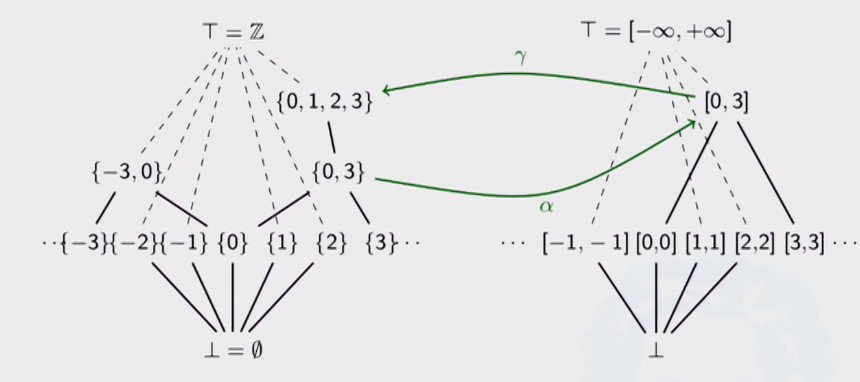
\includegraphics[width=0.6\textwidth]{imagens/abstracao.png}
		\caption[Exemplo da função de Abstração e Concretização]{Exemplo da função de Abstração e Concretização.}
		\fonte{Retirado da apresentação de \citeonline{galoi}.}
		\label{fig:abstracao}
	\end{center}
\end{ilustracao}

Formalmente, define-se que a partir de um estado abstrato \textit{s}, $\gamma$ (s) representa o conjunto de possíveis concretizações que podem ocorrer a \textit{s}. Já um estado concreto S, sua função $\delta$(S) corresponde a um único estado abstrato. Em outras palavras, um estado abstrato pode representar diferentes estados concretos, enquanto que um estado concreto representa um único estado abstrato. Alterações de um estado ocorrem constantemente, e são representadas por $\Delta$, ou \textit{diff}, sendo ele a mudança sofrida de um estado para outro. Em outras palavras, o estado S atualizado para o estado S' sofre a diferença $\Delta$, portanto, S' $=$ S + $\Delta$. 

As funções de transformação de domínio $\gamma$ e $\delta$ podem ser aplicadas não somente nos estados, mas também nas diferenças entre estados. $\gamma$($\delta$), por exemplo, expressa a abstração de uma \textit{diff} $\delta$ qualquer, enquanto $\delta$ representa a concretização da \textit{diff} $\delta$. Algumas conclusões podem ser estabelecidas sobre as \textit{diff}, como $\gamma$(S') $=$ $\gamma$(S) + $\gamma$($\delta$) se S'$=$ S + $\Delta$. Sendo $\alpha$ a representação de uma abstração de uma \textit{diff} $\Delta$ aplicada ao estado S, pode-se deduzir que $\Delta$ $\in$ $\gamma$(S, $\alpha$($\Delta$)) e para cada $\Delta$´ $\in$ $\gamma$(S, $\alpha$($\Delta$)) obtém-se $\alpha$(S $+$ $\Delta$´) $=$ $\alpha$(S´).


\subsection{Aplicação dos estados}

No Protocolo de Integridade de Semântica Segura (SSIP), representam-se as informações do servidor e do cliente em estados, que podem ser tanto abstratos quanto concretos. A representatividade destes estados pode ser encontrada na implementação realizada, referenciada no Capítulo \ref{cap:desenvolvimento}. 

Neste protocolo, o servidor principal da aplicação é denominado Servidor de Estados, que equivale a um servidor convencional de uma NVE, implementado para interagir com os usuários e estabelecer comunicações e trocas de dados sobre as informações do jogo. O servidor de estados contém um estado central abstrato ASTATE, que contém informações relevantes de todos clientes. Imaginando o estado ASTATE como um vetor, por exemplo, cada uma de suas partes é relevante para um cliente conectado a ele. Em outras palavras, de todo estado ASTATE, apenas a parcela ASTATE[$cli_i$] é relevante para o cliente $cli_i$.

Como os clientes possuem estados concretos das informações do jogo, e o servidor possui apenas uma versão abstrata disso,
as funções de transposição de domínios apresentadas no capítulo \ref{cap:definicaoestado} acabam ocorrendo constantemente na comunicação cliente-servidor. Exceto na primeira mensagem de inicialização do cliente com o servidor, por exemplo, todas mensagens posteriores enviadas pelo cliente passam pela função de transposição de abstração. Estas abstrações das mensagens do cliente existem para amenizar o excesso de processamento gerado no servidor nos testes que executa para verificar a validade da mensagem. 

Um exemplo simplificado deste caso encontra-se no jogo implementado \textit{Shooterman} (capítulo \ref{shoterman}). Enquanto variáveis como posição são mantidas no servidor, variáveis de controle mais refinado das ações do personagem são mantidas unicamente no cliente de jogo, como por exemplo, o tempo de recarga de suas ações. Essas informações do estado do jogador são mais abstraídas para o servidor, enquanto são concretas para o cliente do jogador.

Em cada um dos ciclos do cliente, ele envia ao servidor uma abstração $\gamma$ $=$ $\alpha$($\Delta$), que contém uma abstração da \textit{diff} dos últimos estados. Esta abstração é denominada \textit{diff de requisição}. Após o recebimento da \textit{diff} de requisição, o servidor valida a mensagem de acordo com suas semânticas pré-estabelecidas e retorna ao cliente uma confirmação das mudanças requisitadas e das atualizações realizadas pelos outros clientes conectados a NVE. 

Utilizando esta técnica, um cliente malicioso ainda pode violar as regras semânticas estabelecidas pelo servidor, pela susceptibilidade do protocolo, afinal ele só pode verificar se as atualizações abstratas são consistentes com o estado abstrato, sem levar em consideração os valores concretos avaliados. Para solucionar esta falha, ciclos de auditoria são utilizados constantemente para verificar as atualizações de acordo com os estados concretos dos clientes conectados.

\subsection{SSIP}
Outro servidor, denominado Servidor de Auditoria, é utilizado para verificar a integridade semântica dos estados que são constantemente atualizados pelos clientes. Este servidor requisita a um cliente sua sequência de atualizações de estados concretos de um tempo específico junto com seu estado concreto inicial completo, e a partir deles, computa os estados em ordem, verificando sua integridade.

Uma série de operações devem ser seguidas na comunicação do cliente com o servidor de auditoria, e \cite{NVE} dividiu estas operações em três diferentes protocolos, que são apresentados a seguir. Nas ilustrações dos protocolos, são utilizados as setas $\rightarrow$ que representam pacotes enviados de forma não-confiável, e as setas $\hookrightarrow$, que representam pacotes enviados de forma confiável.

\subsection{Protocolo de Inicialização}
\label{protocoloinicializacao}

Este protocolo ocorre quando o cliente inicia seu contato com o servidor. A Figura 3.2 mostra a sequência de passos que deve ser tomada no início da comunicação do cliente com o servidor do jogo.

\begin{figure}[h!]
	\begin{center}
		\fbox{\begin{minipage}{30em}
		\begin{enumerate}
		\small
		\item cli inicializa \textit{t} $:=$ 0 e envia requisição de solicitação ao servidor de estado
		\item Servidor de estado $\rightarrow$ servidor de auditoria : \textit{k} $:=$ GeraMac($1^{n}$)
		\item Servidor de auditoria $\rightarrow$ cli : \textit{h} $:=$ GeraHash($1^{n}$)
		\item Servidor de estado escolhe o estado S do conjunto ASTATE 
		\item Servidor de estado $\rightarrow$ cli: AuthMsg(\textit{k}, S $\parallel$ $n_0$, cli)
		\item cli define $S_0$ como S.
		\item cli $\hookrightarrow$ servidor de auditoria: $Q_0$ $:=$ $CFHash_h$($S_0$)
		\end{enumerate}

		\end{minipage}}

	\end{center}
	\fonte{Traduzido de \cite{NVE}. Protocolo Initialize}
	\caption[Definição do Protocolo de Inicialização.]{Definição do Protocolo de Inicialização.}
	\label{fig:inicializar}	
	
\end{figure}

Primeiramente, o cliente inicializa a variável \textit{t}, que representa o número do ciclo em que ele se encontra. No passo 2, o servidor de estado envia ao servidor de auditoria a variável \textit{k}, que representa uma chave criptográfica. Essa chave criptográfica é gerada usando o \textit{Message Authentication Code} (MAC), algoritmo que recebe como entrada uma chave secreta e uma mensagem a ser autenticada, gerando uma MAC, ou etiqueta.\cite{mac}

No terceiro passo, define-se \textit{h}, índice que representará qual função \textit{hash} o cliente utilizará posteriormente em suas mensagens enviadas a auditoria. O parâmetro \textit{n} da função GeraHash representa o nível de segurança da \textit{hash}. 

Em seguida, o servidor envia uma mensagem ao cliente contendo o estado S escolhido no quarto passo, e o cliente a define como seu estado primário $S_0$. A mensagem é enviada junto com a etiqueta MAC gerada.

No começo de cada auditoria, o cliente envia ao servidor de auditoria uma \textit{hash} de seu estado concreto completo. Apesar do custo computacional ser relativamente alto, dependendo do tamanho da informação contida em um estado concreto, a mensagem precisa chegar entre os próximos \textit{n} ciclos do cliente. O último passo deste protocolo demonstra o envio do estado concreto $S_0$ ao servidor de auditoria. Após o envio, a inicialização é finalizada.


\subsection{Procotolo de Atualização dos Status}

Este protocolo é executado em cada ciclo do cliente. Ele consiste na atualização do estado do cliente após a confirmação do servidor,

Além de manter seu estado concreto atual, o cliente mantém seus estados anteriores em um \textit{buffer} local, contendo até três estados completos e 3\textit{n} \textit{diffs} geradas ao longo de sua execução. Enquanto novos estados e suas \textit{diffs} são inseridas no \textit{buffer}, seus conteúdos antigos podem ser removidos por não serem mais úteis no protocolo. Essas características do \textit{buffer} correspondem a um processo semelhante ao de uma janela deslizante, onde as informações relevantes que o \textit{buffer} armazena são sempre as mais recentes. Todas mensagens recebidas do servidor de auditoria também são armazenadas no cliente de acordo com o intervalo de tempo determinado pela janela deslizante de seu \textit{buffer}.

\begin{figure}[h!]
	\begin{center}
		\fbox{\begin{minipage}{30em}
		\begin{enumerate}
		\small
		\item cli computa a mudança $\Delta_{\textit{t}+1}$ e gera uma nova abstração $\delta_{\textit{t}+1}$ 
		\item cli $\rightarrow$ servidor de estado$:$ $\delta_{\textit{t}+1}$
		\item Servidor de estado computa a atualização $\delta '_{\textit{t}+1}$ e atualiza ASTATE
		\item Servidor de estado $\rightarrow$ cli$:$ $M_{\textit{t}+1}$ $:=$ AuthMsg(\textit{k}, $\delta_{t+1}$ $\parallel$ 
		$\textit{n}_t$ + 1, cli)
		\item cli armazena $\Delta_{\textit{t}+1}$ e computa $S_{t+1}$ $=$ $S_t$ $+$ $\Delta '_{t+1}$
		\item cli $\hookrightarrow$ servidor de auditoria $:$ $D_{t+1}$ $:=$ $Hash_h$($\Delta '_{t+1}$)
		\item cli incrementa variável \textit{t}
		\item caso \textit{t} mod \textit{l} $=$ 0
			\begin{enumerate}
				\small
				\item cli deleta todos \textit{diffs} $\Delta '_{t-i}$
				\item cli armazena $S_t$ e começa a computar $Q_t$ $:=$ $Hash_h$ ($S_t$)
			\end{enumerate}

		\end{enumerate}

		\end{minipage}}
		\fonte{Traduzido de \cite{NVE}. Protocolo StatusUpdate}
		\caption[Definição do Protocolo de Atualização dos Status.]{Definição do Protocolo de Atualização dos Status.}
		\label{fig:atualizacao}
	\end{center}

		
\end{figure}

No início de cada atualização, o cliente gera a mudança $\Delta$ de acordo com sua ação, gerando uma abstração $\delta$ que é então enviada ao servidor de estado. Ele computa esta atualização a partir da abstração recebida, atualizando seu ASTATE. Após isso, ele envia uma mensagem de confirmação ao cliente com sua etiqueta MAC para identificar sua autenticidade como servidor.

Confirmada a mudança $\Delta$ gerada pelo cliente, ele atualiza seu novo estado, agora sendo $S_{t+1}$, como o passo 5 representa. A partir do tipo de \textit{hash} definido no protocolo anterior de atualização realizado anteriormente declarado na variável \textit{h}, o cliente gera um \textit{hash} dessa mudança $\Delta$ e envia ao servidor de auditoria. O cliente incrementa o número de ciclos armazenado em \textit{t}, e verifica se \textit{t} é múltiplo de \textit{l}. Se for, ele remove todas \textit{diffs} mais antigas geradas anteriormente, além de armazenar seu estado concreto, computar a \textit{hash} deste estado, e enviá-la ao servidor de auditoria.

\subsection{Procotolo de Auditoria}
\label{protocoloAuditoria}

É no protocolo de auditoria que se verifica a validade de um cliente em um certo período de tempo onde ele envia suas mensagens. O primeiro passo, como observado na Figura \ref{fig:auditoria}, é enviar uma mensagem ao cliente convocando-o a uma auditoria, juntamente com o índice $t_0$ que representará o índice inicial das ações que serão enviadas.

\begin{figure}[h!]
	\begin{center}
		\fbox{
			\begin{minipage}{30em}
			\begin{enumerate}
			\small
			\item Servidor de auditoria $\rightarrow$ cli $:$  \textit{audit} $\parallel$ $t_0$
			\item cli computa $t_a$ $=$ $\lfloor$ $\frac{t_0}{l}$ $-$ 2 $\rfloor$ \textit{l}
			\item cli $\rightarrow$ servidor de auditoria $:$ $S_{t_a}$ $\parallel$ $\Delta '_{t_a}$ + 1 $\parallel$ ... $\parallel$ $\Delta '_{t_o}$ $\parallel$ $M_{t_a}$ + 1 $\parallel$ ... $\parallel$ $M_{t_0}$


			\item Para \textit{i} $=$ $\textit{t}_a$, ... $\textit{t}_0$ $-$ 1 onde $\hat{S}_{t_a}$ $=$ $S_{t_a}$
				o servidor de auditoria computa	$\hat{S}_{i+1}$ $=$ $\hat{S}_i$ $+$ $\Delta '_{i+1}$ 

			\item Para todo \textit{i} $=$ $t_a$ $+$, ..., $t_0$ o servidor de auditoria determina se $\Delta '_i$ está de acordo com as regras estipuladas

			\item Para todo \textit{i} $=$ $t_a$ $+$, ..., $t_0$, o servidor de auditoria verifica o MAC e a Hash enviadas pelo cli.

			\item Servidor de auditoria compara as \textit{hashs} $S_{t_a}$ com $Q_{t_a}$ e $\hat{S}_{t_a}$ + l com $Q_{t_a}$ + l.
			\end{enumerate}

			\end{minipage}
		}

	\caption[Definição do Protocolo de Auditoria.]{Definição do Protocolo de Auditoria.}

	\fonte{Traduzido de \cite{NVE}. Protocolo Audit} 
	\label{fig:auditoria}
	
	\end{center}
\end{figure}

Quando ciente da abertura da auditoria, o cliente computa $t_a$. Este valor representa o índice do ciclo mais recente que ele começará a enviar. Então o cliente envia as \textit{diffs} das mensagens de $t_a$ até $t_0$. Em outras palavras, todas mudanças que ocorreram em seu estado deste o instante $t_0$ (início da auditoria) até o instante $t_a$ (representado pela fórmula do passo 2) são enviadas ao servidor de auditoria. Além das \textit{diffs}, seu estato concreto também é enviado, juntamente com todas mensagens $M_i$ no mesmo intervalo de \textit{a} a \textit{0}. Estas mensagens são as mensagens de confirmação recebidas pelo servidor de estado no protocolo de Atualização dos Status (vide Figura 3.3, passo 4).

Em um exemplo, supondo que \textit{l} seja 10, ou seja, a cada 10 ciclos do cliente, uma nova \textit{hash} do estado concreto é gerada e enviada ao servidor de auditoria. Na abertura da auditoria, o servidor de auditoria envia ao cliente $t_0$ equivalente a 30. A partir disso, o cliente calcula $t_a$, como no passo 2, resolvendo que $t_a$ = 10. O cliente então envia seu estado concreto do ciclo $t_a$, juntamente com todas \textit{diffs} do ciclo 10 ao 30, e todas mensagens de confirmação M do ciclo 10 ao 30. O servidor de auditoria então descobre todos estados concretos do ciclo 10 ao 30, usando as abstrações recebidas (passo 4). O servidor também verifica se as \textit{diffs} são consistentes com as abstrações $\delta '$(passo 5).

Com isso, usando as mensagens recebidas anteriormente $Q_i$ (vide Figura \ref{fig:inicializar}, passo 7), e $D_i$ (Figura \ref{fig:atualizacao}, passo 6), o servidor de auditoria consegue comparar as abstrações recebidas aplicando-as a $Q_i$ e verificar se equivalem às ações concretas $D_i$. Depois, ele verifica tanto o MAC contido nas mensagens $M_i$ com \textit{i} variando de $t_a$ a $t_i$, quanto as \textit{hashs} das \textit{diffs} $\Delta '$ com as textit{hashs} recebidas anteriormente em D. Depois o servidor de auditoria compara as \textit{hash} dos estados concretos inicial e final recebidas com os estados gerados atráves do passo 4 e transformados em \textit{hash} para esta comparação.
\chapter{Desenvolvimento}
\label{cap:desenvolvimento}

\colorlet{punct}{red!60!black}
\definecolor{background}{HTML}{EEEEEE}
\definecolor{delim}{RGB}{20,105,176}
\colorlet{numb}{magenta!60!black}

\lstdefinelanguage{json}{
    basicstyle=\normalfont\ttfamily,
    numbers=left,
    numberstyle=\scriptsize,
    stepnumber=1,
    numbersep=8pt,
    showstringspaces=false,
    breaklines=true,
    frame=lines,
    backgroundcolor=\color{background},
    literate=
     *{0}{{{\color{numb}0}}}{1}
      {1}{{{\color{numb}1}}}{1}
      {2}{{{\color{numb}2}}}{1}
      {3}{{{\color{numb}3}}}{1}
      {4}{{{\color{numb}4}}}{1}
      {5}{{{\color{numb}5}}}{1}
      {6}{{{\color{numb}6}}}{1}
      {7}{{{\color{numb}7}}}{1}
      {8}{{{\color{numb}8}}}{1}
      {9}{{{\color{numb}9}}}{1}
      {:}{{{\color{punct}{:}}}}{1}
      {,}{{{\color{punct}{,}}}}{1}
      {\{}{{{\color{delim}{\{}}}}{1}
      {\}}{{{\color{delim}{\}}}}}{1}
      {[}{{{\color{delim}{[}}}}{1}
      {]}{{{\color{delim}{]}}}}{1},
}

Antes de implementar os métodos analisados, é necessário definir qual cenário será considerado e qual aplicação será alvo dos métodos. Este capítulo tem como base definir este modelo de jogo e especificar quais atributos foram levados em consideração na produção do \textit{software}. Além disso, este capítulo demonstra como o jogo foi modelado, e como os métodos foram construídos a partir do cenário estabelecido. 

A definição formal de um jogo pode ser compreendida como qualquer atividade que exiga um jogador e regras que devem ser seguidas. A definição de um jogo \textit{online}, por sua vez, pode ser interpretada como um jogo que pode ser jogado utilizando uma rede de computador, possibilitando com que dois ou mais jogadores participem simultaneamente de uma partida mesmo estando em lugares diferentes. Este conceito pode ser aplicado para qualquer \textit{software} de jogo, tanto \textit{single-players} (jogos eletrônicos para um jogador) como \textit{online}.

A definição utilizada neste trabalho consiste em uma aplicação que utiliza troca de mensagens entre cliente e servidor, em que o cliente interage com a aplicação por meio de suas ações no jogo. As ações escolhidas são enviadas ao servidor e informadas aos outros jogadores que estão conectados na partida. Para simplificar a construção do \textit{software} e pela irrelevância para os métodos estudados, o ambiente virtual e gráfico do jogo foi desconsiderado em sua implementação.


\section{Jogo}
\label{shoterman}

O jogo projetado e implementado é um jogo de tiro (mais conhecido no cenário de jogos como \textit{shooter}), subgênero de jogos de ação, chamado de \textit{Shooterman}, em que o foco principal do jogo se encontra nas ações que o personagem executa usando algum tipo de arma. No jogo, cada personagem possui uma arma de longa distância, com a qual pode atirar outros jogadores, derrotando-os, e assim, adquirindo pontos de vitória.

Apesar de \textit{Shooterman} não possuir interface visual, é importante salientar que ele é um jogo com perspectiva \textit{top-down}, estilo de jogo em que a câmera encontra-se acima do mapa e o jogador visualiza o cenário de uma perspectiva superior. Esta distinção é importante para a implementação adequada da movimentação dos jogadores e dos projéteis que irão atirar. Afinal, suas coordenadas devem condizer com a perspectiva da câmera do jogo. A mêcanica básica do jogo consiste na interação de vários jogadores no mesmo cenário, podendo se movimentar e atirar entre si, e bloquear tiros que estão chegando ao seu alcance. Tanto o escudo que bloqueia os tiros, como os tiros em si possuem um tempo de recarga, prevenindo que os jogadores utilizem constantemente o escudo ou atirem diversos tiros em um curto espaço de tempo. O último jogador que sobreviver no cenário é o vencedor.


\begin{figure}[h!]
  \begin{center}
    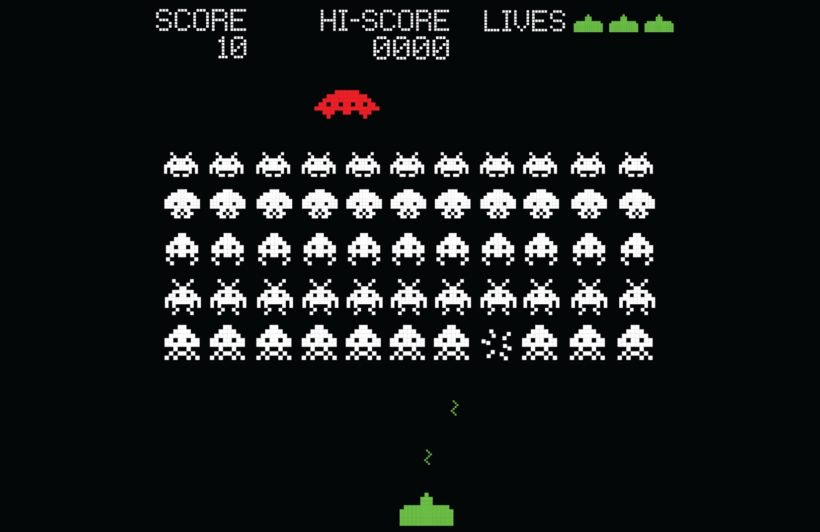
\includegraphics[width=0.6\textwidth]{imagens/space_invaders.jpg}
    \caption{Gameplay do clássico Space Invaders - Exemplo de jogo com câmera top-down.}
    \label{fig:space} 
  \end{center}
\end{figure}


\subsection{Ações do Jogador}

Cada jogador controla um único personagem, que pode atirar projéteis, bloqueá-los e movimentar-se pelo mapa.

O jogador pode movimentar-se em um cenário bidimensional em quatro direções ortogonais - esquerda, direita, baixo e cima. Sempre que ele se movimenta para uma direção, a direção atual que ele está olhando é atualizada. Esta direção será a direção que os projéteis que ele atirar irão seguir.

 A ação principal do personagem é o seu tiro. Quando atira, um projétil é criado a partir de sua posição e atravessa o cenário até colidir com algum objeto ou exceder seu deslocamento máximo. Sempre que o personagem atira, ele não pode atirar novamente por um determinado intervalo de tempo - sua habilidade encontra-se em tempo de recarga.

 O personagem pode também ativar um escudo, uma manobra defensiva, que dura um determinado período de tempo, prevenindo o jogador de ser atingido por ataques inimigos. Este escudo também possui um tempo de recarga que deve ser respeitado.

 Nenhuma dessas ações pode ser executada em um mesmo intervalo de tempo, ou seja, movimentar-se enquanto atira ou atirar enquanto utiliza seu escudo são ações inválidas de acordo com as regras estabelecidas.  



\subsection{Implementação}

Duas aplicações foram implementadas na linguagem C++ versão 11: a versão do cliente e a versão do servidor. Na implementação de \textit{Shooterman}, a autenticidade das mensagens, tanto do cliente quanto do servidor, não foram levadas em consideração da implementação dos métodos. Apesar da transmissão de pacotes utilizar o protocolo UDP, a falha do envio de pacotes também foi descartada para simplificar a implementação dos métodos e avaliar suas funções primárias.


Todas ações executadas pelos jogadores foram enviadas do cliente ao servidor em um \textit{json}. Foi utilizada a biblioteca \textit{JSON for Modern C++}, para facilitar a criação de \textit{jsons} e sua desconstrução em dados brutos utilizados na aplicação \cite{json}. 

\begin{ilustracao}[h!]
  \begin{lstlisting}[language=json,firstnumber=1]
  {
    "player_id" : 4,
    "position": {
      "x" : 5,
      "y" : 8,
      "side" : 0
    },
    "shoot" : "false",
    "barrier_on" : "true"
  }
  \end{lstlisting}
  \caption{Estrutura json utilizada}
  \label{fig:json}

\end{ilustracao}

\lstset {
    language=C++,
    backgroundcolor=\color{black!5},
    basicstyle=\footnotesize,
}

A Figura \ref{fig:json} representa o conteúdo dos dados enviados ao servidor. O mesmo padrão é utilizado pelo servidor ao repassar a mensagem para os outros jogadores, que recebem o arquivo e atualizam as informações do jogo de acordo os dados recebidos. A variável \textit{position} é responsável por representar a posição geográfica do personagem e o lado que ele se encontra. \textit{Shoot} e \textit{barrier\_on} são booleanos de controle que verificam se o jogador está atirando ou ativando sua barreira. \textit{Player\_id} faz referência ao id do jogador que está realizando sua ação. 

No servidor, a classe principal \textit{Game} verifica a cada instante de tempo se um novo cliente conectou-se na aplicação. Sempre que uma nova conexão inicia-se, uma instância da classe \textit{Connection} é criada, onde ela dispara uma \textit{thread} para processar a nova comunicação cliente-servidor, enquanto paralelamente a \textit{thread} principal continua averiguando por novas conexões. A Figura \ref{fig:mainServer} representa a conexão utilizando a classe ServerSocket. Caso o server aceite o novo socket, uma conexão é criada e adicionada a lista de conexões, e uma \textit{thread} é disparada na função newPlayerConnection().

\begin{ilustracao}
    \begin{lstlisting}

        while (true){
            ServerSocket* new_sock = new ServerSocket();
            server->accept (*new_sock);

            try {
                Connection* con = new Connection(this, new_sock, client_id);
                client_connections.push_back(con);
                cout << "Cliente " << client_id  << " conectado!" << endl;
                con->newPlayerConnection();
                client_id++;
            }
            catch (SocketException&) {
                cout << "Erro na conexao com cliente" << endl;
            }
        }
    \end{lstlisting}
    \caption{Thread principal do servidor}
    \label{fig:mainServer}
\end{ilustracao}

Logo quando uma conexão é estabelecida, o servidor envia ao cliente a posição de seu personagem, junto com seu id que será utilizado para identificar seu personagem dentre os outros. Nota-se que o identificador deve ser único para que haja integridade no estado do servidor. Em uma versão mais refinada, em que os clientes cadastram-se na aplicação e possuem seus dados registrados em um banco de dados do servidor, a identificação torna-se mais legítima, afinal, os jogadores teriam seus identificadores únicos registrados junto com informações de suas contas, e utilizariam o mesmo identificador para diversas partidas realizadas na aplicação. Na versão atual, entretanto, os identificadores são provisórios e só se limitam a uma única conexão.

A classe \textit{Connection} é responsável pela comunicação com o cliente conectado, com sua \textit{thread} recebendo mensagens do cliente e retornando suas requisições. Sempre que uma nova mensagem é recebida, ela é validada e enviada a todos jogadores se for considerada semanticamente correta. Percebe-se que dependendo da implementação utilizada no servidor, a função \textit{msgIsValid} varia. Em um cenário que o cliente não possui nenhuma autoridade sobre suas ações, a função avaliaria todas condições necessárias para a ação ser executada, checando sua integridade, e permitindo a ação caso a considerasse legítima. Na versão base da aplicação, entretanto, só é avaliado se o personagem que está realizando a ação realmente é o mesmo controlado pelo usuário da conexão, a partir de seu identificador id. A Figura \ref{mainserver} ilustra a função de comunicação, com a \textit{thread} executando as operações da função update.


\begin{ilustracao}
    \begin{lstlisting}
    void Connection::update(){
      while (true){
        std::string received\_msg;
        *(server_socket) >> received_msg;

        *(player_log) << received_msg << endl;

        auto msg\_json = json::parse(received_msg);
        if (msgIsValid(msg_json) == true){
          updatePlayer(msg_json);
          game->sendToClients(msg_json);
        }
        else{
          cout << "usuario invalido" << endl;
        }
      }
    }
    \end{lstlisting}
    \caption{Função update da classe Conexão responsável pela comunicação cliente servidor}
    \label{mainserver}
\end{ilustracao}


No cliente, a classe principal da aplicação que controla basicamente seu fluxo de operações também é a \textit{Game}. Todos \textit{inputs} do usuário, bem como as comunicações existentes com o servidor operam nesta classe, semelhantemente a classe \textit{Connection} do servidor. Em cada ciclo de execução do cliente, a classe \textit{Game} cuida para que todas suas informações sejam enviadas ao servidor, e que a resposta dele juntamente que contém informações de outros clientes sejam interpretadas e executadas na aplicação.

Sempre que o jogador pressiona uma tecla para atirar, e o cliente pode atirar,  a classe \textit{Game} garante que essa informação seja submetida ao servidor. Essas ações e as verificações que a própria aplicação do cliente faz são executadas na classe \textit{Player}. Esta classe basicamente avalia as ações executadas pelo cliente, e possibilita suas execuções. A classe, por exemplo, verifica se o jogador pode usar seu escudo, ou se ele se encontra indisponível por ter sido utilizado recentemente. Algumas funções e variáveis importantes são ilustradas na Figura \ref{fig:clienteCode1}.

\begin{figure}

  \begin{lstlisting}
  private:
    void toServer();
    void shoot();
    void barrier();
    void checkCooldown();
    void createBullet();

    int side;
    int id;
    bool is_dead = false;
    bool barrier_on = false, can_barrier = true;
    bool can_shot = true, shot = true;

    int shield_cooldown = 0;
    int shot_cooldown = 0;

    const int max_shot_cooldown = 5;
    const int max_shield_cooldown = 15;
    const int shield_time = 5;
    const int player_movespeed = 3;
  \end{lstlisting}

  \caption[Exemplo do arquivo-interface da classe Player da aplicação do cliente.]{Exemplo do arquivo-interface da classe Player.}
  \label{fig:clienteCode1}  

\end{figure}

Todos objetos existentes no jogo, ou mesmo novos objetos que podem ser adicionados futuramente, herdam da classe \textit{GameObject}, que basicamente utiliza a classe \textit{Position}, possibilitando a movimentação dos objetos pelo cenário.

No jogo, somente uma ação pode ser executada por vez, e ações que estiverem em tempo de recarga estarão desabilitadas. Propositalmente, estes testes são verificados no próprio cliente do jogo, então, modificando-o, o cliente pode burlar essas regras, e por exemplo, atirar tiros em um intervalo de tempo menor do que o correto, ou usar seu escudo mais frequentemente que seus adversários.

Todas ações executadas por um cliente são armazenadas em um arquivo, que por sua vez, são analisados com alguns dos métodos estudados no Capítulo 3.


Para facilitar a implementaçãos dos métodos e poder analisar somente seu tempo de processamento, utilizou-se um histórico de mensagens, contendo mensagens enviadas de um cliente ao servidor referente as suas ações executadas. 

\section{Implementação com Execução Simbólica}

\label{implementsimbolic}

Para implementar uma verificador simbólico, deve-se construir uma execução simbólica sobre a aplicação alvo. Visando facilitar os testes e a identificação do custo computacional das verificações das mensagens do cliente, elas foram armazenadas em um arquivo chamado \textit{log}. Neste arquivo, estão armazenadas todas ações executadas por um cliente ao longo de \textit{n} ciclos, onde \textit{n} é o número de linhas do arquivo, e em cada linha dispõe-se a ação realizada. Para gerar o \textit{log}, rodou-se a aplicação do cliente e do servidor durante vários minutos, fazendo com que o cliente faça ações aleatórias em cada um de seus ciclos, enquanto o servidor as armazena no arquivo \textit{log}. Assim, construiu-se uma sequência de ações válidas no arquivo \textit{log}, que foi lida pelo executável simbólico criado. Esta estratégia simula a validação das mensagens do cliente a partir de seu \textit{log} gerado, ou seja, é uma verificação posterior às ações realizadas pelo jogador. Para melhorar o desempenho deste tipo de estratégia, pode-se rodar o algoritmo em apenas parte do \textit{log} armazenado, ou quando se desconfia de um cliente específico após evidências negativas dele vindas de outros clientes. 


O programa usado para gerar a execução simbólica de \textit{Shooterman} foi KLEE, uma máquina virtual simbólica que é construída sobre a estrutura de um compilador LLVM, e disponível gratuitamente\footnote{www.klee.com}. KLEE é baseado em um resolvedor de restrições STP, que implementa uma lógica para encontrar a solução dos conjuntos de restrições impostas a variáveis através da execução simbólica. Para facilitar sua instalação, o KLEE foi utilizado em uma imagem do Docker\footnote{https://www.docker.com/}. Docker é uma plataforma \textit{Open Source} que facilita a criação e administração de ambientes isolados. A partir da imagem obtida do KLEE, foi possível criar um container, contendo o necessário para a utilização das ferramentas e bibliotecas disponíveis da máquina virtual simbólica.  


Para o programa ser executado na máquina simbólica, ele deve primeiramente ser compilado como um arquivo \textit{bitcode} no formato LLVM. Para isso utilizou-se o Clang++, com a \textit{flag} -emit-llvm.  Como vários arquivos são utilizados, usou-se o \textit{llvm-link} para permitir que vários arquivos \textit{bitcode} LLVM juntem-se em um único arquivo \textit{bitcode} \footnote{https://llvm.org/docs/index.html}. Infelizmente, apesar do KLEE reconhecer o arquivo \textit{bitcode} gerado como válido, ele não reconheceu chamadas externas de funções e construtores de outras classes, retornando uma falha de chamada externa logo na construção da primeira classe instanciada.

Para prosseguir com a implementação, o código criado foi modificado para ser compatível em C. Para facilitar essa modificação, somente os arquivos mais essenciais do controle do fluxo do jogo foram convertidos, ocupando o único arquivo 
\textit{client\_main.cpp}. Como a biblioteca \textit{JSON for Modern C++} não pôde ser utilizada, rodou-se um \textit{script} em Python para converter os dados no formato \textit{json} em um formato mais prático de ser lido em C. O A partir deste novo arquivo, pode-se ler linha por linha do arquivo, atribuindo os valores lidos para variáveis usando a função \textit{sscanf} do C. 

Na implementação, somente a variável \textit{action} é representada simbolicamente. Nota-se que na Figura \ref{fig:clienteCodeSimbolica}, a variável \textit{action} representa uma ação que o jogador tomou. Como torna-se simbólica, ela pode representar qualquer valor, variando de 0 a 5, refletindo consequentemente uma das ações possíveis realizadas pelo jogador. A função \textit{randomMovement()} desta implementação atualiza as informações do personagem de acordo com a ação realizada. Basicamente, ela executa a ação passada como parâmetro (a variável simbólica \textit{action}) e determina se o resultado da ação é equivalente com os resultados armazenados na variável \textit{line}. Como a ação é simbólica, considera-se que todas ações possíveis do jogador foram testadas, e se uma delas resultou na equivalência com a ação registrada no log, a ação registrada no log é considerada semanticamente autêntica.

 O retorno dessa função \textit{randomMovement()} retorna a validação da ação. Como cada valor possível de \textit{action} cria um novo ramo de execução, o ramo deve ser finalizado se mostrar-se inválido semanticamente, por isso a função é retornada caso aquela ação seja considerada inválida. Os valores válidos, entretanto, continuam executando e ramificando novamente, na próxima iteração do \textit{while}.

\begin{figure}[h!]
    \begin{lstlisting}
        while ((read = getline(&line, &len, file)) != -1){
            klee_make_symbolic(&action, sizeof(action), "action");
            if (randomMovement(action, line) == false)
                return;
        }
    \end{lstlisting}
    \caption{Exemplo do código de execução simbólica usando KLEE.}
    \label{fig:clienteCodeSimbolica}  

\end{figure}

Em cada iteração do código da Figura \ref{fig:clienteCodeSimbolica}, o próprio KLEE gera restrições sobre a ação \textit{action} executada, determinando se ela deve ser ignorada ou não. Como todas ações possíveis são verificadas, o número de restrições aumenta conforme o número de possibilidades que o jogador poderia executar em cada um de seus ciclos. Na abordagem utilizada, o número de restrições continua a aumentar conforme o número de ações é verificado, fazendo com que o número de ramos de execução gerados seja muito grande, contendo informações duplicadas de possíveis ramos que acabarma falhando em identificar a próxima ação executada. 


\section{Implementação do SSIP}
\label{implementsemantic}

A partir da definição de estados abstratos e concretos do Capítulo \ref{cap:definicaoestado}, pode-se comparar as informações enviadas ao servidor de \textit{Shooterman} como abstratas e as informações contidas no cliente como concretas. Levando em consideração, por exemplo, o escudo que o jogador pode ativar para tornar-se imune aos projéteis inimigos, o servidor somente tem acesso a informação da ativação do escudo, e não de seu tempo de recarga. Em jogos mais complexos, outras informações associadas às ações do jogador, como colisões que podem ocorrer durante uma movimentação do personagem, também podem ser consideradas como informações concretas. Mas, se estas ações fossem enviadas diretamente ao servidor e verificadas lá em cada um dos ciclos do cliente, ocasionariam um processamento extensivo demais para ser realizado pelo servidor. 

Como a autenticidade dos usuários não foi levada em consideração, o uso de \textit{hashs} e autenticadores de mensagens foi desconsiderado tanto na implementação quanto nos custos atribuídos a utilização deste método. 

Analisando o SSIP, percebe-se que para realizar a verificação dos estados do cliente, o servidor de auditoria deve possuir acesso ao estado concreto inicial do cliente (referente ao Protocolo de Inicialização, Capítulo \ref{protocoloinicializacao}), acesso a todas \textit{diffs} entre os estados concretos de $t_a$ a $t_0$, assim como acesso a todas \textit{diffs} entre os estados abstratos de $t_a$ a $t_0$.

Modificando o cliente, foi criado um arquivo durante sua conexão com o servidor, que armazena informações dos estados concretos, \textit{diffs} abstratas e \textit{diffs} concretas de todos estados ao longo de uma partida. 
Este histórico de estados é então lido por um programa, que na prática atua como um servidor de auditoria. Após ler os conteúdos correspondentes aos estados e $\Delta$'s, os passos do protocolo de auditoria (mais detalhes no Capítulo \ref{protocoloAuditoria}) foram executados para verificar a integridade dos estados. 

Primeiramente, a partir do estado concreto inicial, são calculados todos estados concretos a partir das \textit{diffs} concretas obtidas. 
Como todos estados foram armazenados no formato \textit{json}, foi relativamente fácil de atribuir as mudanças $\Delta$ aos estados. A figura \ref{clientestep} ilustra o processo do quarto passo do protocolo de auditoria do Capítulo \ref{protocoloAuditoria}. A figura \ref{fig:exa} ilustra a forma abstrata e concreta de definir informações do jogo. Na primeira linha, é informado a nova posição do jogador após sua movimentação. Informações adicionais, como o tempo de recarga atual de outras habilidades só é retratado nas mensagens concretas, como a segunda linha demonstra. 


\begin{figure}
    \begin{lstlisting}
        auto a = concrete_states.begin();

        next_states.push_back((*a));

        auto delta = concrete_delta.begin();
        string actions[] = {"position", "barrier", "can_barrier", "shield_cooldown", 
        "shoot", "can_shot", "shot_cooldown"};

        for (delta; delta != concrete_delta.end(); delta++){
            json new_state;

            json delta_json = (*delta);

            for (string s : actions){
                if (delta_json.count(s) != 0){
                    new_state[s] = delta_json[s];
                }
            }

            next_states.push_back(new_state);
        }

    \end{lstlisting}
    \caption[Exemplo de criação dos estados a partir do estato concreto e $\Delta$ concretos.]{Exemplo de criação dos estados a partir do estato concreto e $\Delta$ concretos.}
    \label{clientestep}  
\end{figure}


\begin{figure}
  \begin{lstlisting}[language=json,firstnumber=1]
    {"position":{"side":0,"x":-8,"y":8}}
    {"position":{"side":0,"x":-8,"y":8},"shield_cooldown":1}
  \end{lstlisting}
  \caption{Exemplo de diffs abstratas e concretas}
  \label{fig:exa}
\end{figure}


A parte que demanda maior custo computacional deste protocolo é o quinto passo, onde é verificado se cada $\Delta$ concreto é válido ou não. Neste modelo, a partir de cada estado do jogo, é verificado se as ações executadas condizem com a integridade e as regras que a NVE deve cumprir. Ou seja, para cada mudança concreta ocorrida, é analisado se ela poderia ter ocorrido ou não, ou se outra mudança deveria ocorrer no lugar. Um exemplo simples disso seria da utilização da barreira. Caso ela tenha sido usada em um ciclo anterior, os próximos \textit{diffs} concretos devem manter a atualização do tempo de recarga da barreira, até ela poder voltar a ser utilizada. Se o tempo de recarga não apareceu entre uma \textit{diff} e outra após o cliente ter usado sua barreira, ou se a diferença do tempo de recarga entre uma \textit{diff} e outra é maior do que um, conclui-se que o jogador está escondendo informações ou modificando os dados no cliente de jogo.
\chapter{Resultados}
\label{cap:resultados}

Como abordado no Capítulo \ref{cap:desenvolvimento}, os métodos de validação com execução simbólica e o SSIP foram implementados a partir do jogo \textit{Shooterman} criado a fim de analisar estes métodos e estudar seus comportamentos e aplicações.
Todos experimentos foram executados 10 vezes, de onde obteve-se uma média aritmética de seus tempos de execução. Ambos métodos foram avaliados utilizando uma estrutura de arquivo contendo a sequência de ações realizadas por um cliente, facilitando assim o acesso aos dados de tempo de execução do processamento de validação em si, desconsiderando-se as falha de pacotes, latência da rede e outras características que poderiam alterar o tempo total de execução do método.

A máquina usada para os experimentos possui um processador \textit{quad-core} Intel(R) i5-2500 CPU, com 3.30GHz. O sistema operacional utilizado foi o Debian 4.6.2-2. A versão do compilador gcc utilizada foi a 6, e a do clang foi a 3.4.
Para gerar sequências de mensagens inválidas, alterou-se os arquivos de sequências de ações salvas durante uma sessão do jogo \textit{Shooterman}, adicionando ações de ativação de barreira e ativação de tiros em situações que não poderiam ser ativadas. Mudanças como múltiplas ações em uma única mensagem enviada também foram implantadas nos arquivos.

Ambos métodos conseguiram encontrar trapaças em todas as sequências de ações experimentadas. Em situações onde, por exemplo, o usuário atira em um intervalo de tempo que deveria ser proibido pela regras da aplicação, ambos métodos conseguiram reconhecer a trapaça. Situações semelhantes aconteceram quando o usuário tentou ativar seu escudo em momentos que ele estava em tempo de recarga. Outras trapaças, como modificação inválida da posição do jogador também foram reconhecidas pelos métodos.

Para a obtenção do tempo de execução da verificação de execução simbólica, foi utilizado o comando \textit{time} durante o período de execução do programa.
Para a verificação com o sistema de auditoria, foi utilizada a biblioteca \textit{chrono} do C++, possibilitando calcular somente o tempo de processamento das verificações, desconsiderando-se o tempo de leitura do arquivo com as ações verificadas. Esta estratégia foi adotada para ser mais fiel ao protocolo de auditoria, onde o processamento de verificação dos estados do cliente não acontece sobre arquivos armazenados no disco, mas sim sobre os dados já armazenados em memória. 



\section{Resultados da Execução Simbólica aplicada em Shooterman}

Percebe-se que apesar de ser uma implementação simples de execução simbólica, o tempo de execução de verificação das mensagens aumentou consideravelmente de acordo com o número de verificações realizadas. Isto provavelmente se deve ao fato de existir uma quantidade significativa de restrições existentes repetindo o mesmo fluxo de processamento executado pelas restrições anteriores. Ou seja, quando uma terceira ação vai ser validada, por exemplo, o mesmo processo de validação da primeira ação e da segunda ação que já foram calculados, são calculados novamente. 

Para uma sequência pequena a ser validada de 100 ações, o tempo de execução para a comparação foi de 1.5 segundos, valor já considerado alto para uma pequena quantidade de dados. Conforme o número de ações a ser validado aumenta, como o Gráfico \ref{fig:resultsimb} ilustra, o tempo de validação aumenta drasticamente, principalmente após a marca de 600 ações, onde a etapa de validação chega a passar de três minutos. 
Pode-se concluir que quanto mais restrições geradas pela execução simbólica, maior se torna o custo para computar seus próximos ramos. Uma solução para otimizar o custo para resolver de uma sequência grande de restrições pode ser a alteração do algoritmo resolvedor de restrições STP, visando reduzir o número de execuções duplicadas dos ramos. Outra estratégia que pode ser adotada para melhorar o desempenho da execução simbólica na validação das ações de um cliente é a verificação de sequências menores de ações. Como o número de restrições acaba sendo menor, o tempo total acaba sendo bem menor comparado a sequências maiores, como as apresentadas neste trabalho. 

Caso o verificador encontre uma sequência de mensagens inválidas, ele automaticamente para por não encontrar nenhum ramo de execução válido para seguir a computação. Esta abordagem para verificar as mensagens não se mostrou otimizada, e requer outras abordagens para ter um custo computacional menor para ser relevante na verificação de mensagens de jogos \textit{online}.

\begin{grafico}[h!]
	\begin{center}
		\scalebox{0.8}{
			% GNUPLOT: LaTeX picture with Postscript
\begingroup
  \makeatletter
  \providecommand\color[2][]{%
    \GenericError{(gnuplot) \space\space\space\@spaces}{%
      Package color not loaded in conjunction with
      terminal option `colourtext'%
    }{See the gnuplot documentation for explanation.%
    }{Either use 'blacktext' in gnuplot or load the package
      color.sty in LaTeX.}%
    \renewcommand\color[2][]{}%
  }%
  \providecommand\includegraphics[2][]{%
    \GenericError{(gnuplot) \space\space\space\@spaces}{%
      Package graphicx or graphics not loaded%
    }{See the gnuplot documentation for explanation.%
    }{The gnuplot epslatex terminal needs graphicx.sty or graphics.sty.}%
    \renewcommand\includegraphics[2][]{}%
  }%
  \providecommand\rotatebox[2]{#2}%
  \@ifundefined{ifGPcolor}{%
    \newif\ifGPcolor
    \GPcolorfalse
  }{}%
  \@ifundefined{ifGPblacktext}{%
    \newif\ifGPblacktext
    \GPblacktexttrue
  }{}%
  % define a \g@addto@macro without @ in the name:
  \let\gplgaddtomacro\g@addto@macro
  % define empty templates for all commands taking text:
  \gdef\gplbacktext{}%
  \gdef\gplfronttext{}%
  \makeatother
  \ifGPblacktext
    % no textcolor at all
    \def\colorrgb#1{}%
    \def\colorgray#1{}%
  \else
    % gray or color?
    \ifGPcolor
      \def\colorrgb#1{\color[rgb]{#1}}%
      \def\colorgray#1{\color[gray]{#1}}%
      \expandafter\def\csname LTw\endcsname{\color{white}}%
      \expandafter\def\csname LTb\endcsname{\color{black}}%
      \expandafter\def\csname LTa\endcsname{\color{black}}%
      \expandafter\def\csname LT0\endcsname{\color[rgb]{1,0,0}}%
      \expandafter\def\csname LT1\endcsname{\color[rgb]{0,1,0}}%
      \expandafter\def\csname LT2\endcsname{\color[rgb]{0,0,1}}%
      \expandafter\def\csname LT3\endcsname{\color[rgb]{1,0,1}}%
      \expandafter\def\csname LT4\endcsname{\color[rgb]{0,1,1}}%
      \expandafter\def\csname LT5\endcsname{\color[rgb]{1,1,0}}%
      \expandafter\def\csname LT6\endcsname{\color[rgb]{0,0,0}}%
      \expandafter\def\csname LT7\endcsname{\color[rgb]{1,0.3,0}}%
      \expandafter\def\csname LT8\endcsname{\color[rgb]{0.5,0.5,0.5}}%
    \else
      % gray
      \def\colorrgb#1{\color{black}}%
      \def\colorgray#1{\color[gray]{#1}}%
      \expandafter\def\csname LTw\endcsname{\color{white}}%
      \expandafter\def\csname LTb\endcsname{\color{black}}%
      \expandafter\def\csname LTa\endcsname{\color{black}}%
      \expandafter\def\csname LT0\endcsname{\color{black}}%
      \expandafter\def\csname LT1\endcsname{\color{black}}%
      \expandafter\def\csname LT2\endcsname{\color{black}}%
      \expandafter\def\csname LT3\endcsname{\color{black}}%
      \expandafter\def\csname LT4\endcsname{\color{black}}%
      \expandafter\def\csname LT5\endcsname{\color{black}}%
      \expandafter\def\csname LT6\endcsname{\color{black}}%
      \expandafter\def\csname LT7\endcsname{\color{black}}%
      \expandafter\def\csname LT8\endcsname{\color{black}}%
    \fi
  \fi
    \setlength{\unitlength}{0.0500bp}%
    \ifx\gptboxheight\undefined%
      \newlength{\gptboxheight}%
      \newlength{\gptboxwidth}%
      \newsavebox{\gptboxtext}%
    \fi%
    \setlength{\fboxrule}{0.5pt}%
    \setlength{\fboxsep}{1pt}%
\begin{picture}(7200.00,5040.00)%
    \gplgaddtomacro\gplbacktext{%
      \csname LTb\endcsname%
      \put(814,704){\makebox(0,0)[r]{\strut{}$0$}}%
      \csname LTb\endcsname%
      \put(814,1213){\makebox(0,0)[r]{\strut{}$100$}}%
      \csname LTb\endcsname%
      \put(814,1722){\makebox(0,0)[r]{\strut{}$200$}}%
      \csname LTb\endcsname%
      \put(814,2231){\makebox(0,0)[r]{\strut{}$300$}}%
      \csname LTb\endcsname%
      \put(814,2740){\makebox(0,0)[r]{\strut{}$400$}}%
      \csname LTb\endcsname%
      \put(814,3248){\makebox(0,0)[r]{\strut{}$500$}}%
      \csname LTb\endcsname%
      \put(814,3757){\makebox(0,0)[r]{\strut{}$600$}}%
      \csname LTb\endcsname%
      \put(814,4266){\makebox(0,0)[r]{\strut{}$700$}}%
      \csname LTb\endcsname%
      \put(814,4775){\makebox(0,0)[r]{\strut{}$800$}}%
      \put(946,484){\makebox(0,0){\strut{}$128$}}%
      \put(2898,484){\makebox(0,0){\strut{}$256$}}%
      \put(4851,484){\makebox(0,0){\strut{}$512$}}%
      \put(6803,484){\makebox(0,0){\strut{}$1024$}}%
    }%
    \gplgaddtomacro\gplfronttext{%
      \csname LTb\endcsname%
      \put(176,2739){\rotatebox{-270}{\makebox(0,0){\strut{}tempo de execução(s)}}}%
      \put(3874,154){\makebox(0,0){\strut{}nº mensagens}}%
      \csname LTb\endcsname%
      \put(3300,4461){\makebox(0,0)[r]{\strut{}Execução Simbólica}}%
    }%
    \gplbacktext
    \put(0,0){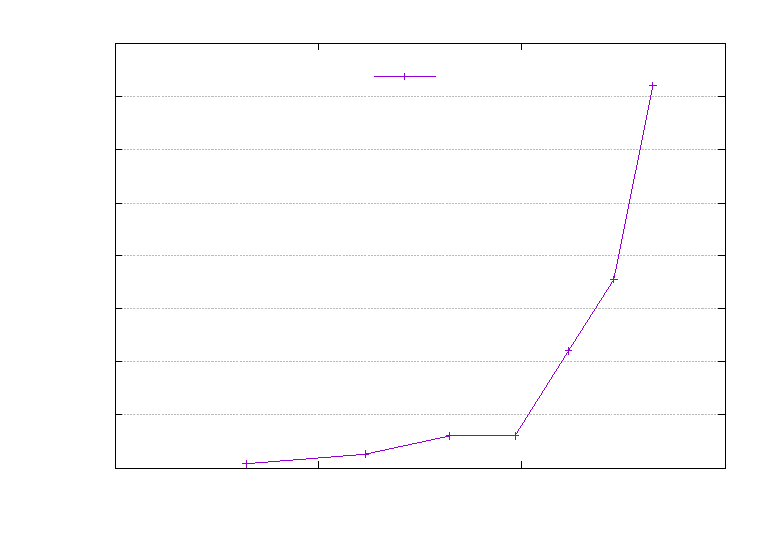
\includegraphics{simbolic}}%
    \gplfronttext
  \end{picture}%
\endgroup
		
			}
		\caption[Resultados obtidos com verificação por execução simbólica.]{Resultados obtidos com validação por execução simbólica.}
		\label{fig:resultsimb}	
	\end{center}

\end{grafico}

\section{Resultados do SSIP aplicado em Shooterman}

Os resultados do protocolo de integridade semântica segura mostraram-se eficientes. Como o Gráfico \label{fig:resultaudit} demonstra, o método conseguiu verificar grandes quantidades de blocos de ações em um curto período de tempo. Para sequências de mensagens com tamanho inferior a 20000, o tempo de execução das verificações foi na escala de microsegundos, com 23 microsegundos de execução tanto para sequências de 10000 e 20000 mensagens. O tempo começou a aumentar em sequências maiores, mas ainda se manteve sempre próximo da faixa de tempo de um segundo. Percebe-se que a cada 10000 novas mensagens a serem processadas, o tempo de execução aumenta aproximadamente 0,15 segundos, mantendo-se em um crescimento linear.  

\begin{grafico}[h!]
	\begin{center}
			%\scalebox{0.8}{
	%		% GNUPLOT: LaTeX picture with Postscript
\begingroup
  \makeatletter
  \providecommand\color[2][]{%
    \GenericError{(gnuplot) \space\space\space\@spaces}{%
      Package color not loaded in conjunction with
      terminal option `colourtext'%
    }{See the gnuplot documentation for explanation.%
    }{Either use 'blacktext' in gnuplot or load the package
      color.sty in LaTeX.}%
    \renewcommand\color[2][]{}%
  }%
  \providecommand\includegraphics[2][]{%
    \GenericError{(gnuplot) \space\space\space\@spaces}{%
      Package graphicx or graphics not loaded%
    }{See the gnuplot documentation for explanation.%
    }{The gnuplot epslatex terminal needs graphicx.sty or graphics.sty.}%
    \renewcommand\includegraphics[2][]{}%
  }%
  \providecommand\rotatebox[2]{#2}%
  \@ifundefined{ifGPcolor}{%
    \newif\ifGPcolor
    \GPcolorfalse
  }{}%
  \@ifundefined{ifGPblacktext}{%
    \newif\ifGPblacktext
    \GPblacktexttrue
  }{}%
  % define a \g@addto@macro without @ in the name:
  \let\gplgaddtomacro\g@addto@macro
  % define empty templates for all commands taking text:
  \gdef\gplbacktext{}%
  \gdef\gplfronttext{}%
  \makeatother
  \ifGPblacktext
    % no textcolor at all
    \def\colorrgb#1{}%
    \def\colorgray#1{}%
  \else
    % gray or color?
    \ifGPcolor
      \def\colorrgb#1{\color[rgb]{#1}}%
      \def\colorgray#1{\color[gray]{#1}}%
      \expandafter\def\csname LTw\endcsname{\color{white}}%
      \expandafter\def\csname LTb\endcsname{\color{black}}%
      \expandafter\def\csname LTa\endcsname{\color{black}}%
      \expandafter\def\csname LT0\endcsname{\color[rgb]{1,0,0}}%
      \expandafter\def\csname LT1\endcsname{\color[rgb]{0,1,0}}%
      \expandafter\def\csname LT2\endcsname{\color[rgb]{0,0,1}}%
      \expandafter\def\csname LT3\endcsname{\color[rgb]{1,0,1}}%
      \expandafter\def\csname LT4\endcsname{\color[rgb]{0,1,1}}%
      \expandafter\def\csname LT5\endcsname{\color[rgb]{1,1,0}}%
      \expandafter\def\csname LT6\endcsname{\color[rgb]{0,0,0}}%
      \expandafter\def\csname LT7\endcsname{\color[rgb]{1,0.3,0}}%
      \expandafter\def\csname LT8\endcsname{\color[rgb]{0.5,0.5,0.5}}%
    \else
      % gray
      \def\colorrgb#1{\color{black}}%
      \def\colorgray#1{\color[gray]{#1}}%
      \expandafter\def\csname LTw\endcsname{\color{white}}%
      \expandafter\def\csname LTb\endcsname{\color{black}}%
      \expandafter\def\csname LTa\endcsname{\color{black}}%
      \expandafter\def\csname LT0\endcsname{\color{black}}%
      \expandafter\def\csname LT1\endcsname{\color{black}}%
      \expandafter\def\csname LT2\endcsname{\color{black}}%
      \expandafter\def\csname LT3\endcsname{\color{black}}%
      \expandafter\def\csname LT4\endcsname{\color{black}}%
      \expandafter\def\csname LT5\endcsname{\color{black}}%
      \expandafter\def\csname LT6\endcsname{\color{black}}%
      \expandafter\def\csname LT7\endcsname{\color{black}}%
      \expandafter\def\csname LT8\endcsname{\color{black}}%
    \fi
  \fi
    \setlength{\unitlength}{0.0500bp}%
    \ifx\gptboxheight\undefined%
      \newlength{\gptboxheight}%
      \newlength{\gptboxwidth}%
      \newsavebox{\gptboxtext}%
    \fi%
    \setlength{\fboxrule}{0.5pt}%
    \setlength{\fboxsep}{1pt}%
\begin{picture}(7200.00,5040.00)%
    \gplgaddtomacro\gplbacktext{%
      \csname LTb\endcsname%
      \put(814,704){\makebox(0,0)[r]{\strut{}$0$}}%
      \csname LTb\endcsname%
      \put(814,1213){\makebox(0,0)[r]{\strut{}$0.1$}}%
      \csname LTb\endcsname%
      \put(814,1722){\makebox(0,0)[r]{\strut{}$0.2$}}%
      \csname LTb\endcsname%
      \put(814,2231){\makebox(0,0)[r]{\strut{}$0.3$}}%
      \csname LTb\endcsname%
      \put(814,2740){\makebox(0,0)[r]{\strut{}$0.4$}}%
      \csname LTb\endcsname%
      \put(814,3248){\makebox(0,0)[r]{\strut{}$0.5$}}%
      \csname LTb\endcsname%
      \put(814,3757){\makebox(0,0)[r]{\strut{}$0.6$}}%
      \csname LTb\endcsname%
      \put(814,4266){\makebox(0,0)[r]{\strut{}$0.7$}}%
      \csname LTb\endcsname%
      \put(814,4775){\makebox(0,0)[r]{\strut{}$0.8$}}%
      \put(946,484){\makebox(0,0){\strut{}$20000$}}%
      \put(1922,484){\makebox(0,0){\strut{}$30000$}}%
      \put(2898,484){\makebox(0,0){\strut{}$40000$}}%
      \put(3875,484){\makebox(0,0){\strut{}$50000$}}%
      \put(4851,484){\makebox(0,0){\strut{}$60000$}}%
      \put(5827,484){\makebox(0,0){\strut{}$70000$}}%
      \put(6803,484){\makebox(0,0){\strut{}$80000$}}%
    }%
    \gplgaddtomacro\gplfronttext{%
      \csname LTb\endcsname%
      \put(176,2739){\rotatebox{-270}{\makebox(0,0){\strut{}tempo de execução(s)}}}%
      \put(3874,154){\makebox(0,0){\strut{}nº mensagens}}%
      \csname LTb\endcsname%
      \put(-1825,3868044){\makebox(0,0)[r]{\strut{}Auditoria}}%
    }%
    \gplbacktext
    \put(0,0){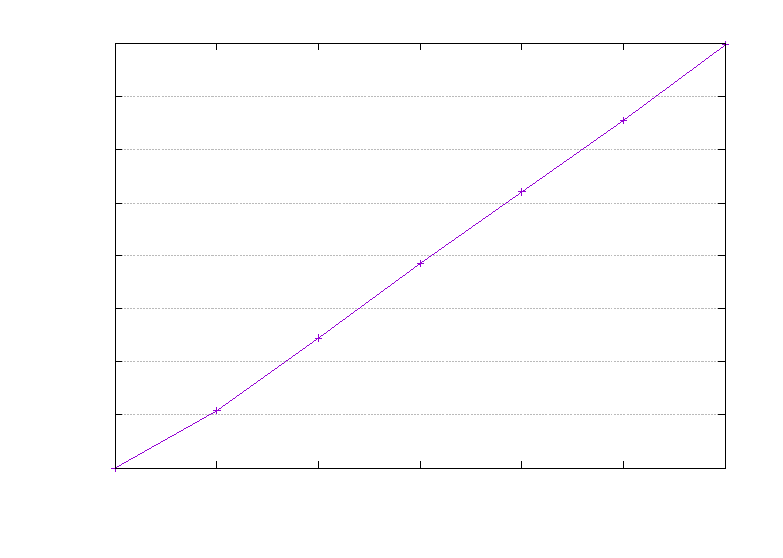
\includegraphics{auditoria}}%
    \gplfronttext
  \end{picture}%
\endgroup
		
	%		}
	    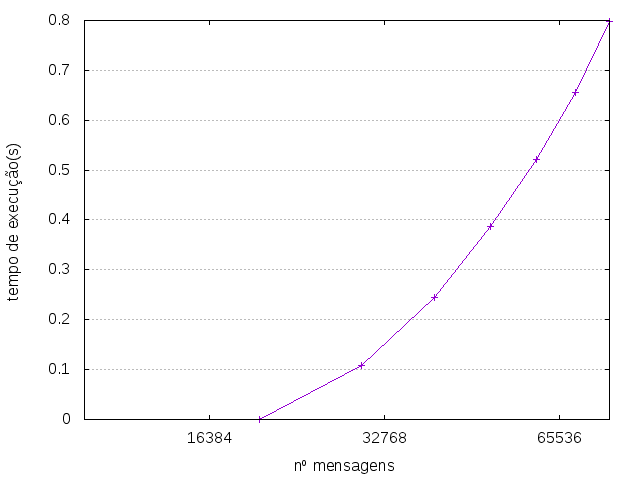
\includegraphics[width=0.65\textwidth]{imagens/auditoria.png}
		\caption[Resultados obtidos com validação com auditoria.]{Resultados obtidos com validação com auditoria.}
		\label{fig:resultaudit}	
	\end{center}

\end{grafico}



Em um cenário convencional, dificilmente o servidor de auditoria precisaria avaliar sequências tão grandes de ações executadas pelo cliente. Mesmo assim, o algoritmo do protocolo mostrou-se eficiente para lidar com sequências de até mesmo 80000 ações. Comparando com os resultados obtidos da verificação de mensagens utilizando execução simbólica, o SSIP mostrou-se muito superior em questões de desempenho de tempo de execução. Além de mostrar-se eficiente na verificação das ações de \textit{Shooterman}, o protocolo mostra-se versátil por dar a opção do desenvolvedor escolher de quantos em quantos ciclos de um cliente inicia-se um processo de auditoria. Além disso, como apenas uma auditoria é feita com um cliente por vez, o processamento gasto pelo servidor de auditoria acaba sendo bem reduzido. No geral, o SSIP mostrou-se interessante para verificar a integridade de mensagens.

Entretanto, algumas características negativas podem ser atribuídas ao SSIP. Considerando que, a cada ciclo do cliente ele envia informações adicionais contendo as mudanças concretas de seus estados ao servidor de auditoria, o número de mensagens a ser enviadas dobra. Além de enviar as alterações abstratas ao servidor da aplicação, as alterações concretas (que possuem tamanhos maiores de mensagens) também são enviadas. Pode-se afirmar, que em média, o tamanho das mensagens do SSIP é o dobro do convencional, pela duplicidade das informações enviadas tanto ao servidor principal como ao servidor de auditoria.


\chapter{Considerações Finais}
\label{cap:conclusao}

Esse projeto teve como propósito estudar diferentes estrátegias de detecção de trapaças em jogos \textit{online}, focando no conjunto de trapaças que envolvem a adulteração do jogo, e analisar suas características. 


Na etapa de desenvolvimento, foi projetado e implementado um pequeno jogo \textit{online} em C++, no modelo cliente-servidor. Este jogo, chamado \textit{Shooterman} foi alvo de dois métodos estudados que verificam as mensagens enviadas pelos clientes, encontrando possíveis usuários trapaceiros e atividades ilegais. Estes dois métodos foram implementados modificando o servidor utilizado no jogo, que verificava sequências de mensagens enviadas por clientes armazenadas em arquivos.

Ao final desta etapa, foi avaliado o desempenho dos métodos baseado no tempo que demoraram para verificar sequências de diferentes tamanhos de mensagens. Ambos métodos conseguiram encontrar sequências inválidas de mensagens enviadas pelo cliente, entretanto, o método que utiliza o protocolo SSIP mostrou-se superior em realizar esta tarefa. O verificador utilizando execução simbólica mostrou-se muito lento, principalmente quando o número de mensagens verificadas passou de 600, levando alguns minutos para realizar esta tarefa.

Como trabalhos futuros, novos métodos de verificação podem ser implementados e analisados com maior profundidade, assim como jogos maiores e complexos podem ser alvo dos métodos, para comparar seus desempenhos em infraestruturas maiores e modelos de ações mais complexos.
         
%\chapter{Conclusão}

%	\par Conclusão do trabalho.
	% \lipsum[1-5]
	
% % % % % % % % % % % % % % % % % % % % % % % % % % % % % % % % % % % % % % 
% % % % % % % % % % % % FIM DAS PAGINAS TEXTUAIS % % % % % % % % % % % % % % 
% % % % % % % % % % % % % % % % % % % % % % % % % % % % % % % % % % % % % % 



% % % % % % % % % % % % % % % % % % % % % % % % % % % % % % % % % % % % % % 	
% % % % % % % % % % % % % BIBLIOGRAFIA  % % % % % % % % % % % % % % % % % % 
% % % % % % % % % % % % % % % % % % % % % % % % % % % % % % % % % % % % % % 	

\bibliografia{referencias}  %%%%% BIBLIOGRAFIA -> INCLUIR NAS CHAVES O NOME DO ARQUIVO *.BIB	
	
	
	
% % % % % % % % % % % % % % % % % % % % % % % % % % % % % % % % % % % % % 	
% % % % % % % % % % % % % APENDICES % % % % % % % % % % % % % % % % % % %
% % % % % % % % % % % % % % % % % % % % % % % % % % % % % % % % % % % % % 	
% 	\apendice %%%% TEXTOS A PARIR DESTE PONTO SERAO CONSIDERADOS APENDICES

% \chapter{Demonstração de algo}
%         \par Algo como apêndice.  
%          \lipsum[2-10]

          
% % % % % % % % % % % % % % % % % % % % % % % % % % % % % % % % % % % % % % 	
% % % % % % % % % % % % % % % ANEXOS  % % % % % % % % % % % % % % % % % % % 
% % % % % % % % % % % % % % % % % % % % % % % % % % % % % % % % % % % % % % 	
\anexo    %%%% TEXTOS A PARIR DESTE PONTO SERAO CONSIDERADOS ANEXOS
\begin{comment}
        
\chapter{Algo interessante que alguém fez}
         \par Algo como anexo.
         \lipsum[2-10]
                  
        \begin{grafico}[ht]
     	    \caption{\label{exepretex2}Orientações para a lombada do trabalho.}
	    \centering
     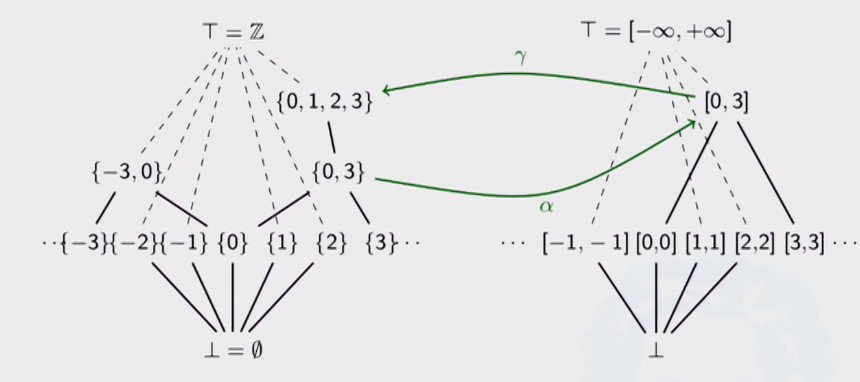
\includegraphics[width=0.6\textwidth]{imagens/abstracao.png}
     \fonte{Adaptado de aaa.}
         \end{grafico}         
         
          \lipsum[2-10]

\end{comment}

         
\end{document}
